\documentclass[cn,11pt,chinese]{elegantbook}

	\title{优雅地用Zotero进行文献管理和论文写作}
	\subtitle{A Short Intrduction to Zotero}
	
	\author{韩敏义}
	\institute{南京农业大学\\\kaishu\hspace{1.1cm}温氏食品集团股份有限公司}
	\date{January 15, 2021}
	\version{1.13}
	%\bioinfo{自定义}{信息}
	%\extrainfo{Victory won\rq t come to us unless we go to it. --- M. Moore}
	
	\logo{logo.jpg}
	\cover{cover.jpg}
	
	% 本文档命令
	\usepackage{array}
	\newcommand{\ccr}[1]{\makecell{{\color{#1}\rule{1cm}{1cm}}}}
	%章节显示调整
	%\renewcommand\thesection{\zhnumber{chapter}.\arabic{subsection}}
	%\renewcommand\thesection{\zhnumber{chapter}.\arabic{section}}
	%\renewcommand\thesection{\zhnumber{section}}
	%\renewcommand{\thesection}{第~\zhnumber{\arabic{section}}~节}
	%package
	\usepackage{cleveref}  
	%改为第X章
	\crefformat{chapter}{#2第\zhnumber{#1}章#3}
	%改为第X节 
	\crefformat{section}{#2第#1节#3}
	%改为第X页 
	\crefformat{page}{#2第#1页#3}
	%图表调整
	\def\figureautorefname{图}%
	\def\tableautorefname{表}%
	
	%修改链接颜色
	\hypersetup{linkcolor=blue,
		citecolor=blue,
		urlcolor=blue}
	
	%修改题注为符号
	\renewcommand*{\thefootnote}{\fnsymbol{footnote}}
	% 修改目录深度
	\setcounter{tocdepth}{2}
	%\usepackage[text={140mm,240mm},centering]{geometry}

	%JavaScript定义
	\lstdefinelanguage{JavaScript}{
		keywords={typeof, new, true, false, catch, function, return, null, catch, switch, var, if, in, while, do, else, case, break},
		keywordstyle=\color{blue}\bfseries,
		ndkeywords={class, export, boolean, throw, implements, import, this},
		ndkeywordstyle=\color{darkgray}\bfseries,
		identifierstyle=\color{black},
		sensitive=false,
		comment=[l]{//},
		morecomment=[s]{/*}{*/},
		commentstyle=\color{purple}\ttfamily,
		stringstyle=\color{red}\ttfamily,
		morestring=[b]',
		morestring=[b]"
	  }
	  
	  \lstset{
		 language=JavaScript,
		 %backgroundcolor=\color{lightgray},
		 extendedchars=true,
		 basicstyle=\footnotesize\ttfamily,
		 showstringspaces=false,
		 showspaces=false,
		 %numbers=left,
		 %numberstyle=\footnotesize,
		 %numbersep=9pt,
		 tabsize=2,
		 breaklines=true,
		 showtabs=false,
		 captionpos=b
	  }
	  
	  \usepackage[parfill]{parskip}
\begin{document}

 
\maketitle
\frontmatter

  \chapter*{内容简介}
		\markboth{Introduction}{内容简介}
	
		文献管理软件对于参考文献的管理、阅读,在论文撰写过程中插入参考文献有很大的帮助作用,其种类有很多,有商业软件,
		如Endnote,NoteExpress等,也有免费开源的,如Zotero,Mendeley等,在试用过很多软件后,发现免费开源的Zotero
		可以很方便的从网上导入文献,管理文献及与Word集成,在撰写文章的时候方便的插入参考文献。Endnote用的人很多,也很
		简单易用,为什么还要学习Zotero呢?最吸引我的在于三个方面,首先,Zotero开源免费,不用再找破解版或license了。
		其次,如果有权限,Zotero在下载题录\footnote{根据\href{https://zhidao.baidu.com/question/443193991.html}
		{百度知道},题录是指文献的基本信息,包括题名、作者、关键词、作者机构、文献来源、摘要等。选择保存题录是指当获得检索结果后,
		如需要将检索结果的目录保存以供他用时,可在检索结果的简单页面上选择条目进行保存。}的同时可以把全文也下载下来,
		并且自动链接到相应题录上\footnote{当前只支持外文的数据库,\href{http://www.cnki.net}{CNKI}等中文的数据库还不支持。
		更新:20200304 使用新的\href{https://github.com/Zotero-CN/translators_CN}{cnki.js}后也可以在导入题录的同时下载中国期刊网的PDF了。
		详见\cref{sec:cnki_fulltext}。};最后,Zotero结合其他的同步盘如\href{https://www.jianguoyun.com}{坚果云}、
		\href{https://office.live.com/start/OneDrive.aspx}{OneDrive}使得在不同电脑间同步题录和全文也变得十分方便。
		因此推荐大家学习一下Zotero的使用。
		\
		如果你只想用Zotero从网上导入题录,请看\cref{ch:install},这章介绍了Zotero的下载安装,从网站导入题录及链接全文。
		如果还想用Zotero在Word中插入参考文献,请看\cref{ch:insert},如果你还有同步题录及全文的需要,请看\cref{ch:syn}。
		如果你加入了学科组,有共享群组文献的需要或从群组库复制文献,请看\cref{ch:group}。一些高级应用请看\cref{ch:questions}。
		
		
		本文档在\href{http://tug.org/texlive/}{\TeX{} Live 2020} 环境下用\href{https://code.visualstudio.com/}{Visual Studio Code}
		中编辑,使用了\href{https://elegantlatex.org/}{ElegantBook的书籍模板}在此致谢;
		如发现问题请反馈至\href{mailto:redleafnew@163.com}{redleafnew@163.com},
		或关注我的知乎专栏\href{https://zhuanlan.zhihu.com/c_1071081428967743488}{软件随心},谢谢。

\tableofcontents
%\listofchanges

\mainmatter
%第一章
\chapter[Zotero下载安装及题录导入]{Zotero下载安装及题录导入\footnote{以下介绍的Zotero都是基于英文界面操作,
  		大家可以方便地根据截图找到相应的中文界面位置。}}\label{ch:install}
	\section{Zotero的安装} 
	Zotero原来是基于Firefox浏览器的一个插件,现在有基于桌面的独立安装版。Zotero支持现在常见的操作系统,
	如Windows、Linux及MacOS。
	可以到\url{https://www.zotero.org/download/}去下载相应操作系统及位数的安装包。
	这里以Windowns 10 64位版本的安装文件为例进行说明。
	\begin{enumerate}
		\item 双击下载的安装文件,如Zotero-x.x.x\_setup.exe(x为具体的版本号,\autoref{fig:package}),
		首先会显示正在解压的界面,如\autoref{fig:extracting}所示,
		如果出现用户帐户控制,点击“是”,如\autoref{fig:userControl}:
		\begin{figure}[htbp]
			\centering
			\begin{minipage}[t]{\dimexpr0.5\textwidth-4em}
				\centering
				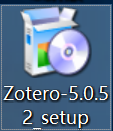
\includegraphics[width=0.3\linewidth]{package}
				\caption{下载的安装包}
				\label{fig:package}
			\end{minipage}
			\begin{minipage}[t]{\dimexpr0.5\textwidth-4em}
				\centering
				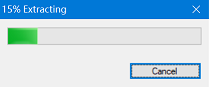
\includegraphics[scale=1.4]{extracting}
				\caption{安装文件解压界面}
				\label{fig:extracting}
			\end{minipage}
		\end{figure}
		
			\item 然后出现安装向导,如\autoref{fig:installwiz1}所示,点击下一步。
				%fig user control
				\begin{figure}[htbp]
					\centering
					\begin{minipage}[t]{\dimexpr0.5\textwidth-4em}
						\centering
						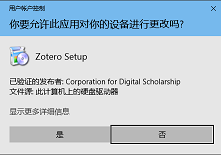
\includegraphics[scale = 1.3]{ch1userControl}
						\caption{用户帐户控制}
						\label{fig:userControl}
					\end{minipage}
					\hspace{1em}		
					\begin{minipage}[t]{\dimexpr0.5\textwidth-4em}
						\centering
						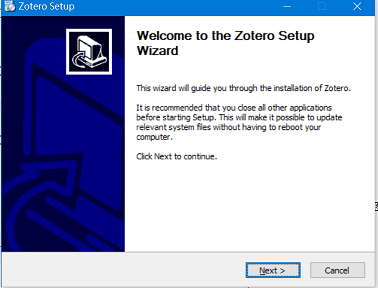
\includegraphics[scale = 0.8]{installwiz1}
						\caption{安装向导第一步}
						\label{fig:installwiz1}
					\end{minipage}
				\end{figure}
			\item 接下来选择安装类型,如\autoref{fig:installType},
			一般选择Standard(标准)就可以,如果有兴趣也可以选择Custom(定制),
			选择Custom在点下一步会提示可以修改安装目录
			(默认安装目录为\path{C:\Program Files (x86)\Zotero} )以及是否在桌面上及
			开始菜单的程序组中放置图标。
			\item 选择Standard后点击下一步提示安装目录为\path{C:\Program Files (x86)\Zotero},
			此处无法修改安装目录,
			如\autoref{fig:ch1StartInstall}。如果要修改需要在上一步选择Custom选项。
			\item 此时信息已经收集完毕,点击Install(安装)就开始安装了,如\autoref{fig:ch1Installing}。
			\item 最后安装完成,点击Finish(完成)就可以打开Zotero,如\autoref{fig:ch1InstallComplete}所示。
			\item 如果觉得安装麻烦,也可以点击
			\href{https://www.zotero.org/download/client/dl?channel=release&platform=win32-zip}{下载Zip格式},
			解压后直接使用。另外,也可以从\href{https://github.com/pedrom34/ZoteroPortable}
			{https://github.com/pedrom34/ZoteroPortable}下载便携格式,下载的方法是在页面上点击绿色的“Code”按钮,
			再点击Download ZIP,下载完毕后解压,运行ZoteroPortable.exe即可打开Zotero,使用也十分方便,甚至可以解压到U盘,
			做到真正的便携。

	\end{enumerate}
		
			\begin{figure}[htbp]
				
				\begin{minipage}[t]{\dimexpr0.5\textwidth-4em}
					\centering
					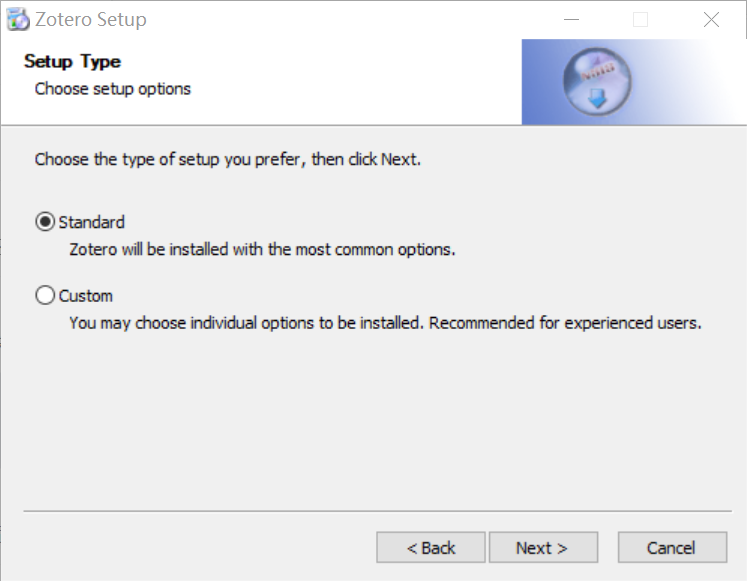
\includegraphics[scale=0.43]{ch1InstallType}
					\caption{选择安装类型}
					\label{fig:installType}
				\end{minipage}
				\hspace{1cm}	
				\begin{minipage}[t]{\dimexpr0.5\textwidth-4em}
						%fig install start
					\centering
					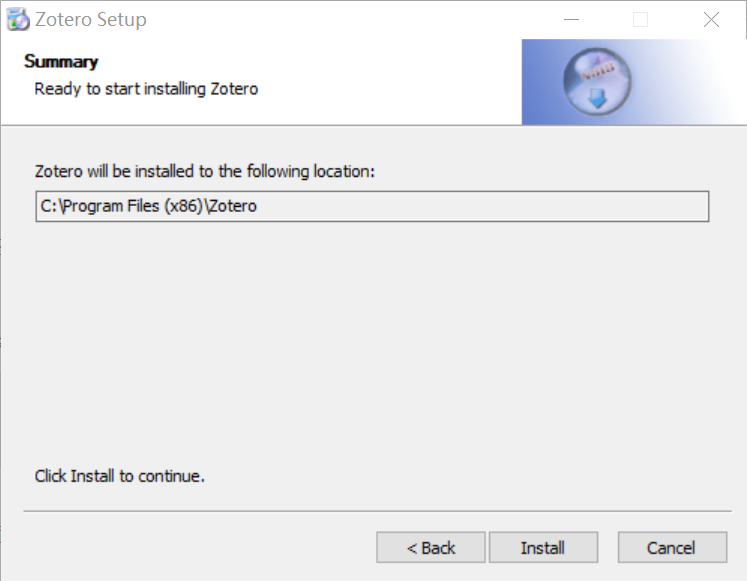
\includegraphics[scale=0.43]{ch1StartInstall}
					\caption{点击Install开始安装}
					\label{fig:ch1StartInstall}
				\end{minipage}
				
			\end{figure}	
		
			
			%fig installing
			\begin{figure}[htbp]
				\noindent
				\begin{minipage}[t]{\dimexpr0.5\textwidth-4em}
					\centering
					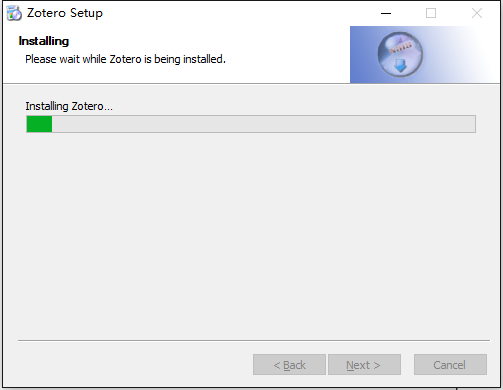
\includegraphics[scale=0.43]{ch1Installing}
					\caption{Zotero正在安装}
					\label{fig:ch1Installing}
				\end{minipage}
				\hspace{1cm}	
				\noindent
				\begin{minipage}[t]{\dimexpr0.5\textwidth-4em}
					%fig install complete
					\centering
					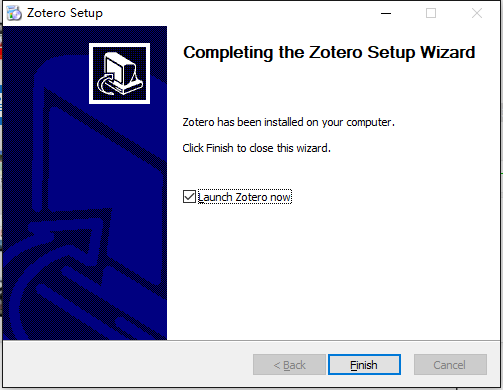
\includegraphics[scale=0.43]{ch1InstallComplete}
					\caption{Zotero安装完成}
					\label{fig:ch1InstallComplete}	
				\end{minipage}
			\end{figure}	
			
		
	\section{浏览器插件的安装} 
	要想快速的导入文献,最好装上Zotero的浏览器插件。
	Zotero针对不同的浏览器(Chrome、Firefox、Safari和最新的Chromium内核的Edge,不支持IE浏览器)
	有不同的插件。	在这里推荐比较好用的Chrome内核浏览器:
	CentBrowser(百分浏览器),可以到\url{http://www.centbrowser.cn/history.html}
	根据自己的操作系统位数,下载安装版或便携版。
	
	在访问\href{https://www.zotero.org/download/}
	{Zotero浏览器插件安装网站https://www.zotero.org/download/}时,
	网站会自动检测当前所用浏览器内核,提示安装相应的插件,
	如\autoref{fig:ch1PluginWeb}所示。可以直接点击Install Chrome Connector,
	然后出现是否需要安装的提示,如\autoref{fig:ch1PluginInstall},
	点击“添加扩展程序”进行插件安装。插件的安装过程有可能需要翻墙,
	成功安装后会在合适的位置根据当前网页的类型显示不同图标,
	一般网页的图标如\autoref{fig:ch1ZoteroIcon}显示,如果没有打开网站,
	则会显示一个灰色的“Z”。
	  
	  如果无法安装,可以到\href{https://pan.baidu.com/s/1SRsAKk6XV8z8ImGueocPNQ}
	{https://pan.baidu.com/s/1SRsAKk6XV8z8ImGueocPNQ}下载针对Chrome内核的插件进行离线安装。
	% browser type
	\begin{figure}[htbp]
		\centering
		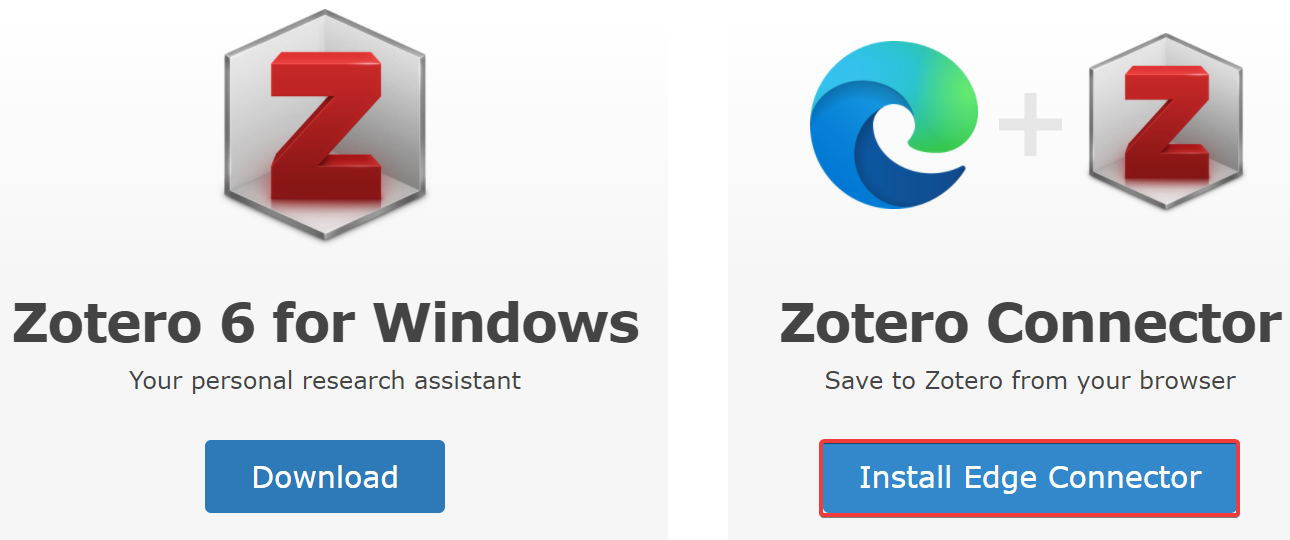
\includegraphics[width=0.6\linewidth]{ch1PluginWeb}
		\caption{Zotero浏览器插件安装网站会自动检测当前浏览器类型}
		\label{fig:ch1PluginWeb}
	\end{figure}
	% install connector
	\begin{figure}[htbp]
		\centering
		
\includegraphics[width=0.6\linewidth]{ch1PluginInstall}
		\caption{浏览器提示是否安装插件(扩展程序)}
		\label{fig:ch1PluginInstall}
	\end{figure}
	%zotero icon
	\begin{figure}[htbp]
		\centering
		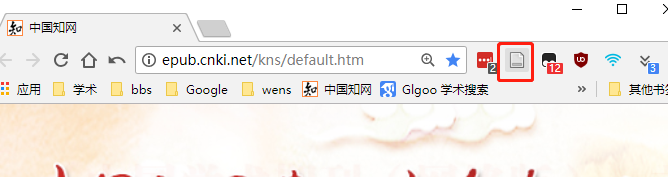
\includegraphics[width=0.8\linewidth]{ch1ZoteroIcon}
		\caption{Zotero浏览器中显示的图标}
		\label{fig:ch1ZoteroIcon}
	\end{figure}
	
	下载后离线安装的方法是,以百分浏览器为例,
	将下载的zotero\_connector\_x.crx(x为版本号)拖入百分浏览器,
	而后浏览器的提示与\autoref{fig:ch1PluginInstall}类似,
	如\autoref{fig:ch1PluginInstall2}。
	%zotero icon
	\begin{figure}[htbp]
		\centering
		
\includegraphics[width=0.7\linewidth]{ch1PluginInstall2}
		\caption{将下载的插件插入到百分浏览器后的提示}
		\label{fig:ch1PluginInstall2}
	\end{figure}
	
	Google 的 Chrome 浏览器宣布从最新Chrome版本开始默认只允许从 Chrome Web Store 
	下载安装扩展程序,网上有一些解决办法,但我没有试成功。
	所以只能翻墙在Chrome的应用商店上下载或是使用修改版的Chrome。
	\section{建立自己的Zotero文献库}\label{sec:newLibrary}
	\subsection{设置文献库在硬盘上的位置} 
	\begin{enumerate}
		\item 
		建立自己的Zotero文献库首先需要选择自己的将要建立文献库在硬盘上的位置,
		方法是在Zotero中依次点击Edit-Preferences,
		如\autoref{fig:ch1ZoteroPre1}所示。
		%data folder
		\begin{figure}[htbp]
			\centering
			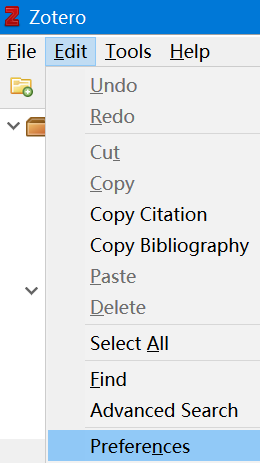
\includegraphics[width=0.5\linewidth]{ch3ZoteroPre1}
			\caption{打开Zotero设置}
			\label{fig:ch1ZoteroPre1}
		\end{figure}
		
		\item 
		在弹出的Zotero Preferences对话框中,依次点击Advanced-Files and Folders,
		设置Base directory为我们存放全文文件夹。
		文献库在Zotero中默认的存贮位置为\path{C:\Users\<Your Name>\Zotero},
		最好我们不要将这些数据不要存放在系统盘,防止系统崩溃造成无法挽回的损失。
		我们可以将这个目录改为自己的文件夹,如\autoref{fig:ch3BaseDir}所示
		%data folder
		\begin{figure}[htbp]
			\centering
			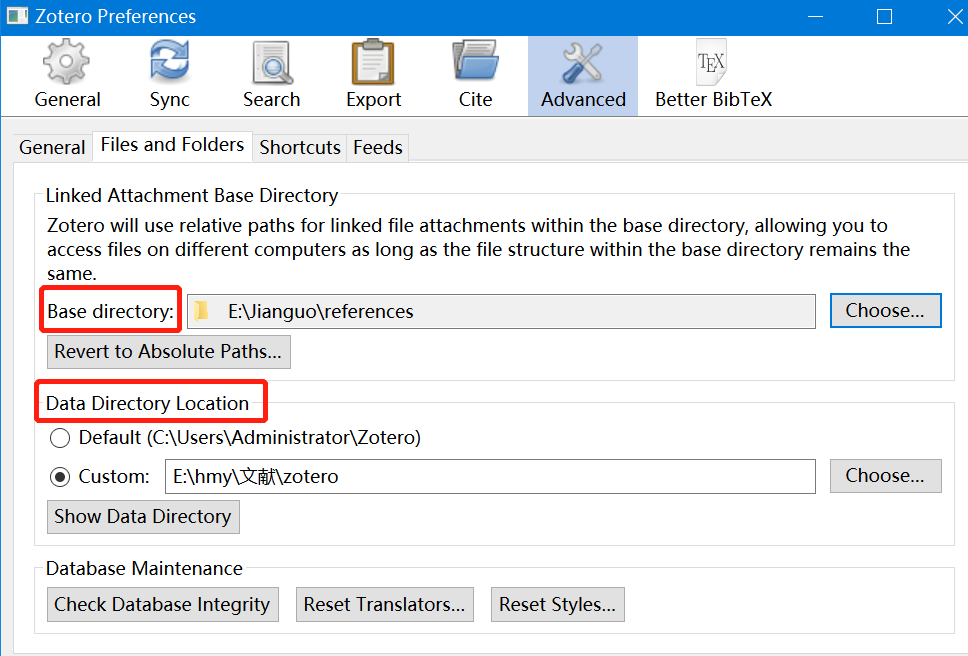
\includegraphics[width=0.8\linewidth]{ch3BaseDir}
			\caption{Zotero文件夹设置}
			\label{fig:ch3BaseDir}
		\end{figure}
		\item \label{sec:creat_folder}
		设置完文献存贮位置后,最好还要在Zotero中根据自己的课题方向或文献的类型等建立不同的分类(文件夹),
		方便对文献进行分类管理。
		建立分类(文件夹)的方法是在Zotero中依次点击File-New Collection...,
		如\autoref{fig:ch1ZoteroNewColl1}所示,或是在Zotero左侧的My library上右击,选择New Collection...,
		在弹出的对话框中输入自己的分类名称,如\autoref{fig:ch1ZoteroNewColl2}所示。
		%New Collection
		\begin{figure}
			\centering
			\begin{minipage}[t]{\dimexpr0.5\textwidth-4em}
				\centering
				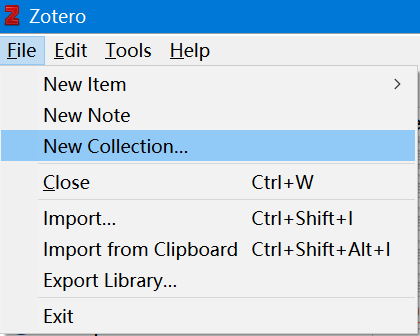
\includegraphics[scale=0.3]{ch1ZoteroNewColl1}
				\caption{在Zotero中新建分类步骤1}
				\label{fig:ch1ZoteroNewColl1}
			\end{minipage}
		   \hspace{1.5cm}
			\begin{minipage}[t]{\dimexpr0.5\textwidth-4em}
				\centering
				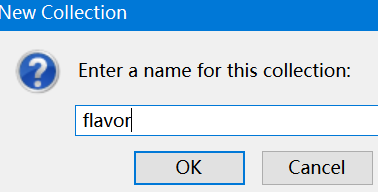
\includegraphics[scale=0.4]{ch1ZoteroNewColl2}
				\caption{在Zotero中新建分类步骤2}
				\label{fig:ch1ZoteroNewColl2}
			\end{minipage}
		\end{figure}
		\item 
		然后就会看到Zotero左侧面板中出现了刚才新建的分类,
		如\autoref{fig:ch1ZoteroNewColl3}所示,可以通过此方法建立多个分类,
		而且可以通过在分类上右击,选择在分类下面再建立子分类,
		如\autoref{fig:ch1ZoteroNewColl4}所示\footnote{除了分类(文件夹之外),还可以通过
		标签和关联对文献进行管理,见\cref{sec:tag}和
		\href{https://zhuanlan.zhihu.com/p/275707703}{Zotero分类、标签和关联的使用。}}。
		
		%New Collection2
		\begin{figure}[htbp]
			\begin{minipage}[t]{0.4\linewidth}
				\centering
				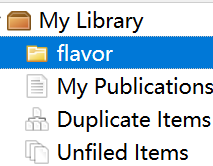
\includegraphics[scale=0.7]{ch1ZoteroNewColl3}
				\caption{在Zotero中新建分类结果}
				\label{fig:ch1ZoteroNewColl3}
			\end{minipage}
			\begin{minipage}[t]{0.7\linewidth}
				\centering
				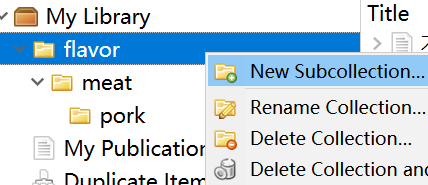
\includegraphics[scale=0.45]{ch1ZoteroNewColl4}
				\caption{可以在Zotero分类中新建子分类}
				\label{fig:ch1ZoteroNewColl4}
			\end{minipage}
		\end{figure}
	\end{enumerate}
	\subsection{从网站导入题录及全文} \label{sec:ImportFromWeb}
	有很多方式可以在Zotero库中添加文献条目,最方便的还是直接在网上数据库进行导入,
	安装浏览器插件(扩展)的目的也正是为此。
	浏览器上Zotero的图标会根据当前打开网页的文献类型而显示不同的图标,
	默认如\autoref{fig:ch1ZoteroIcon}显示,
	当前网页含有多条文献时显示为文件夹图标,如果是学位论文则显示学位帽图标。
	Zotero的这种自动感知功能十分强大,
	期刊的网页我目前还没有碰到过不能感知的。实际上自动感知所支持的网页还有Amazon,Nytimes等,
	而且Zotero支持的网页数目还在持续增长。
	Zotero支持现在常见的网络数据库,如Sciencedirect、Springer及PubMed文献数据库等。我们仅以SD数据库、
	中国知网CNKI和Google Scholar为例看一下。
	\subsubsection{Science Direct文献导入}
	我们完全打开具体的某篇文章的网页时,当鼠标指标Zotero在浏览器中的图标时,
	会提示:Save to Zotero (ScienceDirect), 如\autoref{fig:ch1SDImport}。
	一般括号中会显示当前文献所属的数据库或期刊名称。
	此时,点击这个图标,这篇文献就会导入到Zotero库中,如\autoref{fig:ch1SDRef}。
	比较吸引人的是,如果有这个数据库(期刊)的权限,
	这个篇对应的PDF会同时下载下来,而且链接到这篇文献,在Zotero文献库中双击这个条目,
	则系统会自动调用PDF阅读器打开这篇文献,
	是不是很方便?如果打开文献网页时鼠标指向Zotero在浏览器中的图标时提示
	Save to Zotero (Web Page with snapshot),
	原因是网页还没有完全打开,稍等一会儿或是刷新网页等显示正常了再导入。
	%SD import
	\begin{figure}[htbp]
		\centering
		
\includegraphics[width=0.7\linewidth]{ch1SDImport}
		\caption{导入ScienceDirect数据库时的提示}
		\label{fig:ch1SDImport}
	\end{figure}
	%SD ref
	\begin{figure}
		\centering
		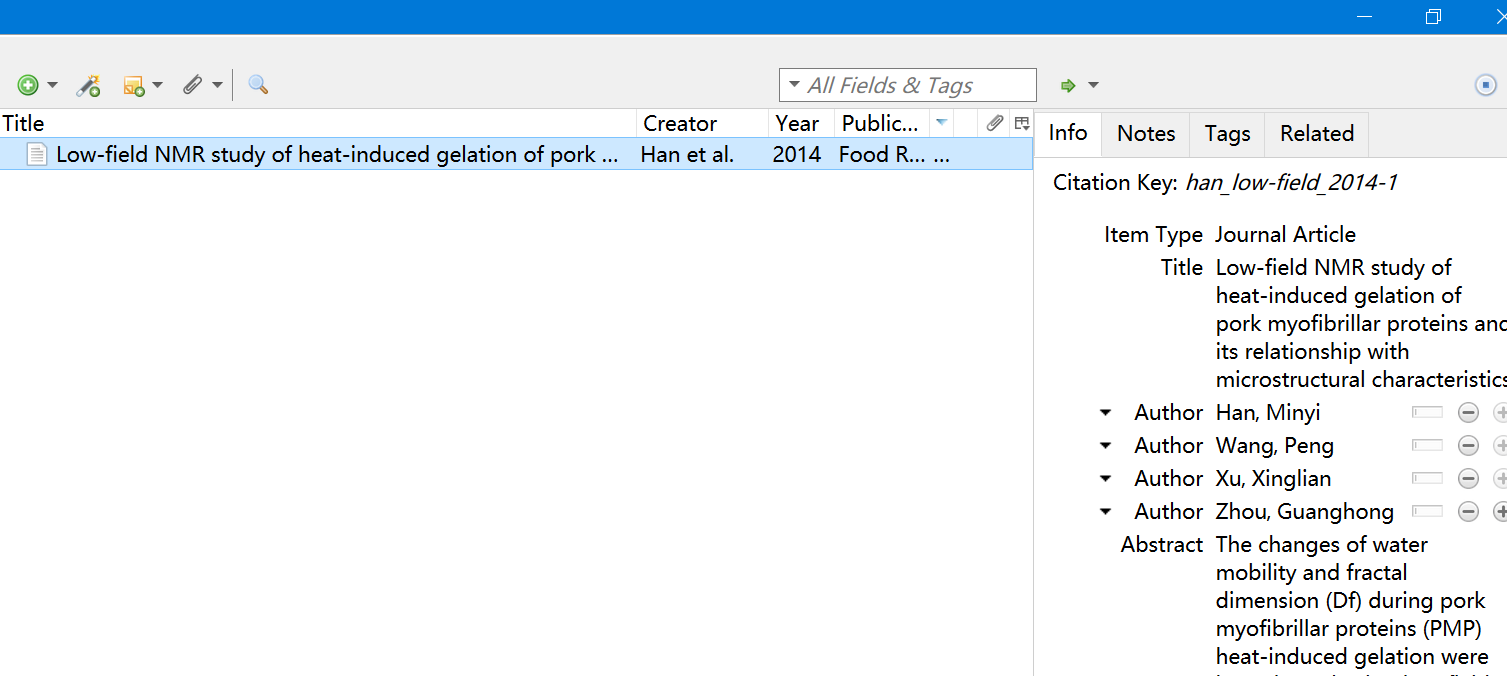
\includegraphics[width=0.7\linewidth]{ch1SDRef}
		\caption{导入的ScienceDirect文献在Zotero库中的显示结果}
		\label{fig:ch1SDRef}
	\end{figure}
	\subsubsection{中国知网文献导入} \label{sec:cnki}
	在中国知网主页\url{http://www.cnki.net/}搜索结果中点击具体的文献,
	打开文献的页面,此时鼠标移向Zotero在浏览器中的图标时,提示Save to Zotero (CNKI),
	如\autoref{fig:ch1CNKIImport},点击这个图标,对应的文献就会导入到Zotero库中,但遗憾的是即使有权限,
	对应的全文CAJ或PDF都不会一起导入\footnote{更新:
	20200304 使用新的\href{https://github.com/Zotero-CN/translators_CN}{cnki.js}
	后也可以下载中国期刊网的PDF了,
	详见\cref{sec:cnki_fulltext}。}。如果\url{http://www.cnki.net/}
	这个网站不好用,可以试试\url{http://epub.cnki.net/kns/default.htm}。
	%CNKI import
	\begin{figure}[htbp]
		\centering
		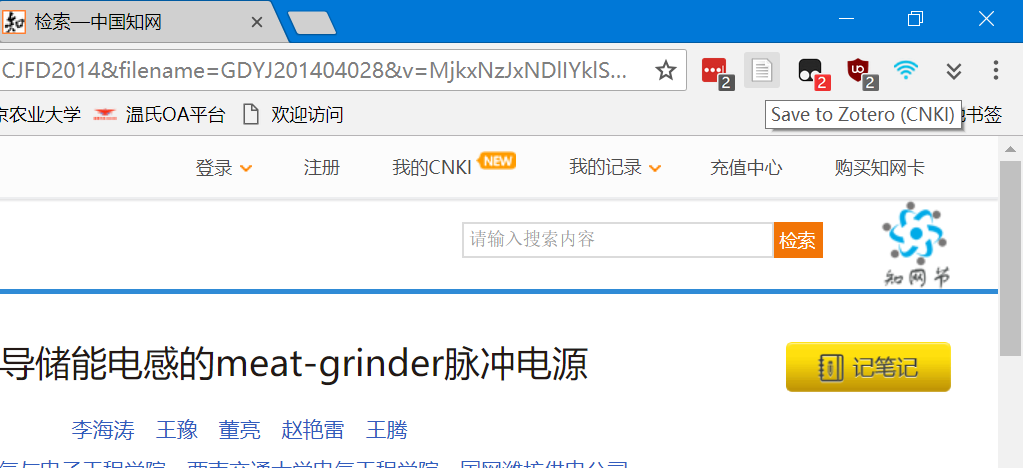
\includegraphics[width=0.7\linewidth]{ch1CNKIImport}
		\caption{导入中国知网数据库时的提示}
		\label{fig:ch1CNKIImport}
	\end{figure}
	\subsubsection{通过Google Scholar导入文献}
	在Google Scholar搜索结果页面中,Zotero在浏览器中图标会变成一个文件夹图标,
	点击这个小图标,在显示的页面中我们可以选择需要的条目,然后点击ok,
	我们选择的条目就会自动导入的Zotero库中。
	但是Zotero的浏览器插件不支持Google Scholar的一些镜像网站(如\url{https://scholar.glgoo.org/})。
	\subsection{通过文献标识符导入题录}
	如果已知文献的ISBN、DOI、PMID或arXiv ID,
	可以通过文献标识符导入到Zotero库中,在Zotero中,点击魔术棒,
	输入这些ID,如DOI:10.1016/j.meatsci.2016.03.026,
	如\autoref{fig:DOI}所示,然后按回车键,则对应的文献就会被导入到库中,
	注意如用这种方式导入文献也需要保持互联网畅通。
	%DOI import
	\begin{figure}[htbp]
		\centering
		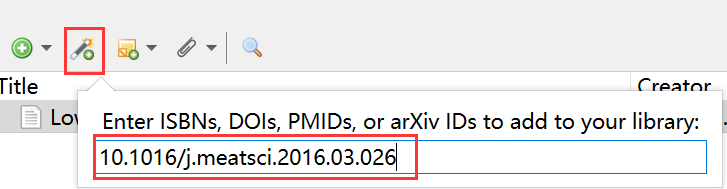
\includegraphics[width=0.7\linewidth]{ch1DOI}
		\caption{通过DOI导入文献}
		\label{fig:DOI}
	\end{figure}

	\subsection{已有PDF文献的导入} \label{sec:EngPDFIm}
	对于以前下载的PDF文献,Zotero也可以很方便地提取PDF的元
	信息(这里PDF的导入是指英文的PDF文件,
	中文PDF的导入方式见\cref{sec:Chinese_PDF}),同时把此PDF作为附件链接到这篇文献中。
	已有PDF文献导入的方式是将PDF直接拖入到Zotero中,
	如\autoref{fig:ch1PDFImport}所示,
	Zotero会自动提取该PDF文件元数据(如文章的作者、题目、年代等信息),
	如\autoref{fig:ch1PDFImport1}所示。
	%PDF import
	\begin{figure}[htbp]
		\centering
		
\includegraphics[width=0.7\linewidth]{ch1PDFImport}
		\caption{直接将PDF文件插入到Zotero中}
		\label{fig:ch1PDFImport}
	\end{figure}
	\begin{figure}[htbp]
		\centering
		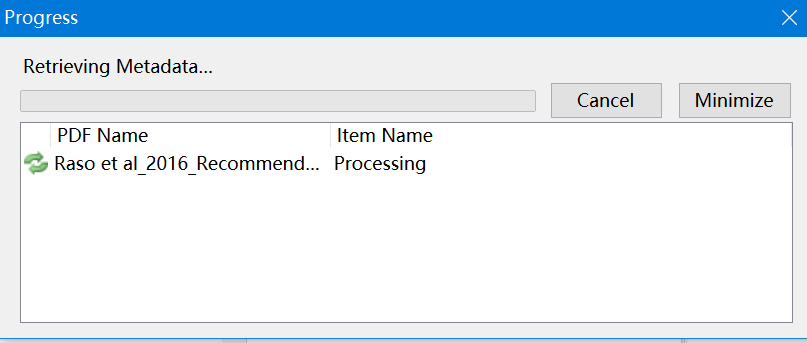
\includegraphics[width=0.7\linewidth]{ch1PDFImport1}
		\caption{Zotero提取PDF元数据}
		\label{fig:ch1PDFImport1}
	\end{figure}
	
	\subsection{从其他文献管理软件导入}\label{OtherRefSoft}
	如果以前用其他文献管理软件或是从其他人的Zotero库中导入,
	Zotero可以方便地导入。首先,从其他文献管理软件导出BibTex、RIS或Zotero RDF格式。
	然后,在Zotero中点击File-Import,
	如\autoref{fig:ch1ImportFromOther}所示
	,根据提示找到导出的文件即可将那些文献导入到Zotero中。
	%imort from other software
	\begin{figure}
		\centering
		\begin{minipage}[t]{\dimexpr0.5\textwidth-4em}
			\centering
			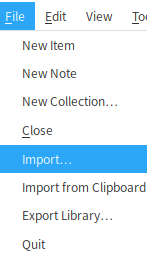
\includegraphics[scale = 1]{ch1ImportFromOther}
			\caption{Zotero导入其他文献管理软件中的数据}
			\label{fig:ch1ImportFromOther}
		\end{minipage}	
		%Manual New refence
		\hspace{1cm}
		\begin{minipage}[t]{\dimexpr0.5\textwidth-4em}
			\centering
			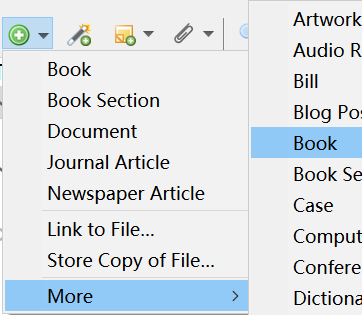
\includegraphics[scale = 0.8]{ch1ManualNew}
			\caption{Zotero中手动添加新文献}
			\label{fig:ch1ManualNew}
		\end{minipage}	
	\end{figure}

	\subsection{手动录入题录}\label{sec:ManualImport}
	对于那些不能从网上找到的文献,如一些老的文献、国家标准、
	会议论文等,只能手动录入文献的信息。手动新建文献的方法是:
	在Zotero界面中点击“+”图标右边的小箭头,
	选择正确的文献类型,如\autoref{fig:ch1ManualNew}所示,
	然后在Zotero右侧填入文献对应的信息,如:题目、作者、年代等信息,
	如\autoref{fig:ch1ManualNewBook}所示。
			%Manual New refence
			\begin{figure}
					\centering
					\begin{minipage}[t]{\dimexpr0.5\textwidth-4em}
					\centering
					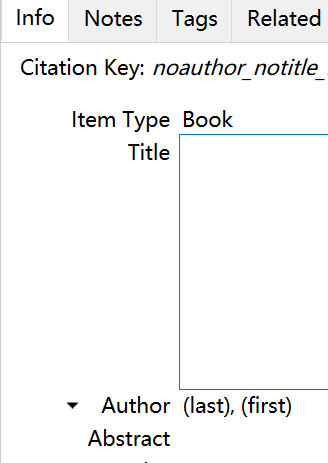
\includegraphics[scale = 0.4]{ch1ManualNewBook}
					\caption{Zotero中新建书籍}
					\label{fig:ch1ManualNewBook}
				\end{minipage}	
				\hspace{2cm}
				%	%link file 
				\begin{minipage}[t]{\dimexpr0.5\textwidth-4em}
					\centering
					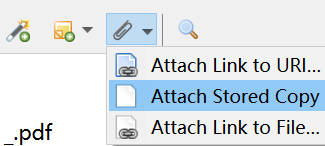
\includegraphics[scale = 0.8]{ch1LinkFile1}
					\caption{Zotero中链接文献}
					\label{fig:ch1LinkFile1}
				\end{minipage}	
			\end{figure}
			%link file2
			\begin{figure}
				\centering
				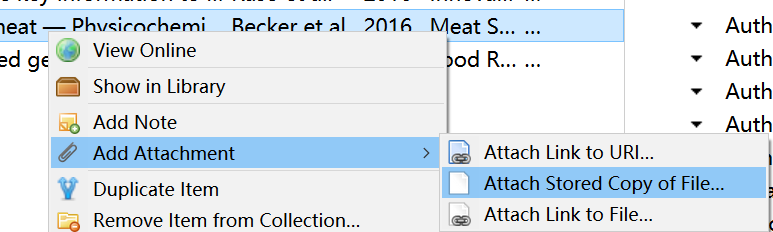
\includegraphics[width=0.7\linewidth]{ch1LinkFile2}
				\caption{通过右击Zotero中链接文献}
				\label{fig:ch1LinkFile2}
			\end{figure}
		\subsection{链接全文}\label{sec:linkFulltex}
				对于我们从其他网站下载的全文或其他附件信息,
				我们可以手动链接到参考文献条目中,方法是先选中对应的参考文献条目
				,在Zotero点击回形针图标,
				选择Attach Stored Copy of File ...,
				如\autoref{fig:ch1LinkFile1}所示,找到相应的附件。
				或在条目上右击,选择Add Attachment,如\autoref{fig:ch1LinkFile2}所示,
				后续步骤与前述相同。链接上附件后,原来存的文件可以删除。
  \chapter{在Word中写作时用Zotero插入参考文献}\label{ch:insert}
		建立了自己的Zotero文献库后,
		在写文章尤其是综述类的文章时就可以方便地利用Zotero插入文献了。
		现在Zotero对于Libre Office中的Writer和MS Office中的Word支持比较好。
		尽管在WPS中会出现Zotero的工具条,但在插入文献时会出现错误。
		本文以Word 2016为例进行讲述。如果安装正确的话,在Word中会形成Zotero的工具条,
		如\autoref{fig:ch2ZotoeroTool}所示,
		主要操作在这个工具条中进行。
		如果在Word中没有出现Zotero的工具条,可以尝试用见\cref{sec:tool_bar}的方法解决。
		 %tool bar
			\begin{figure}[htbp]
				\centering
				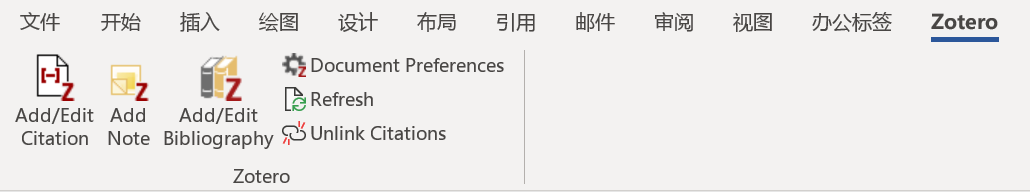
\includegraphics[scale=0.5]{ch2ZotoeroTool}
				\caption{Zotero在Word中工具条}
				\label{fig:ch2ZotoeroTool}
			\end{figure}
		
		\section{插入参考文献}\label{sec:insertRef}
		我们在写文章时,尤其是文章的前言或数据的分析讨论部分及在综述类的文章中往往需要插入参考文献,
		在Word中插入Zotero管理的参考文献的方法比较简单,步骤如下:
		\begin{enumerate}
			\item
			点击Zotero在Word工具条中的第一个按钮Add/Edit Citation,
			在弹出的对话框中选择需要的Style(一般是期刊或数据库的名称),
			点击OK,如\autoref{fig:ch2WordInsert}所示。
			%select style
			\begin{figure}[htbp]
				\centering
				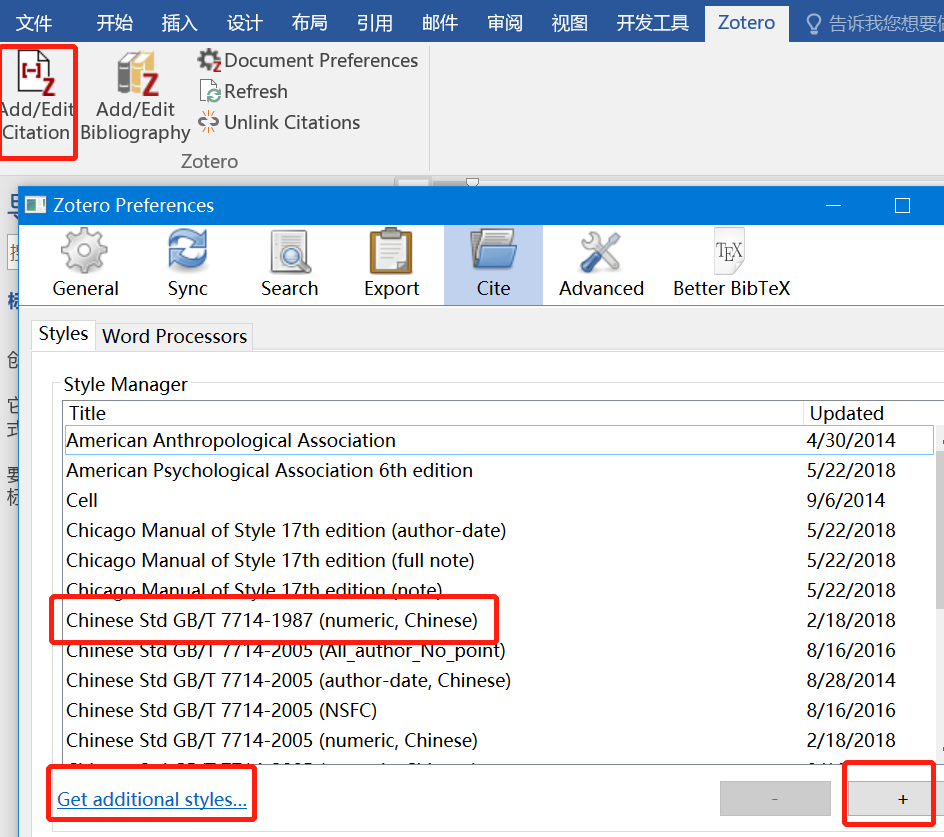
\includegraphics[scale=0.6]{ch2WordInsert}
				\caption{选择需要的Style}
				\label{fig:ch2WordInsert}
			\end{figure}
			\item
			如果列表中没有我们需要的文章格式\label{tag:notyle},
			点击\autoref{fig:ch2WordInsert}中的Manage Styles...,则会弹出Zotero Preferences对话框,
			如\autoref{fig:ch2ZoteroPre}所示。
			%Zotero Preferences
			\begin{figure}[htbp]
				\centering
				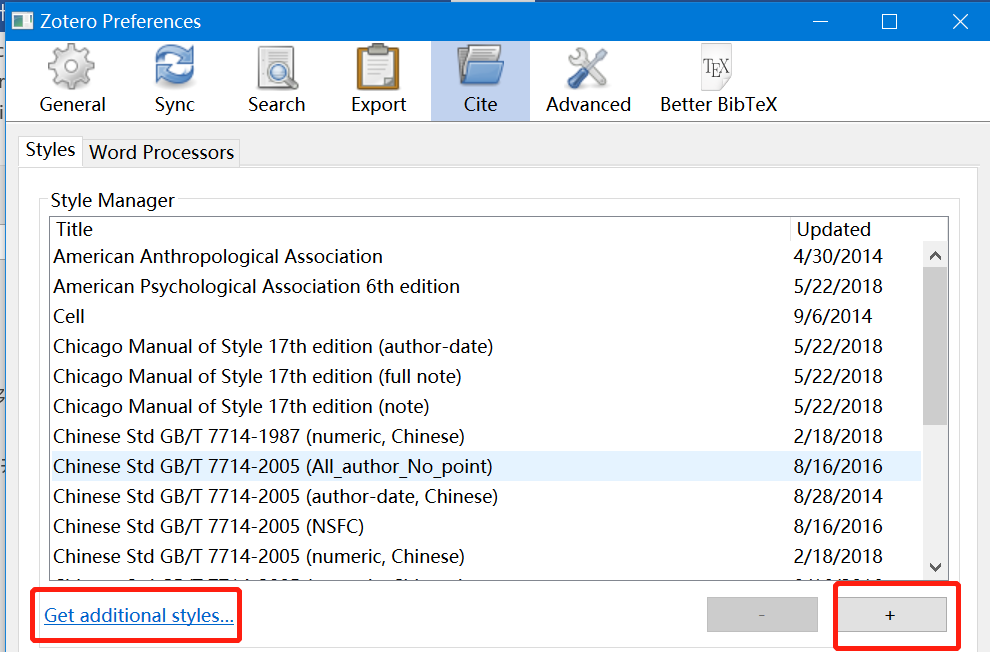
\includegraphics[scale=0.6]{ch2ZoteroPre}
				\caption{Zotero Preferences}
				\label{fig:ch2ZoteroPre}
			\end{figure}
			\item
			点击\autoref{fig:ch2ZoteroPre}中“+”,
			找到从网站上或从其他人那得到的csl文件。
			或是点击Get additional styles...,则会打开Zotero的Style仓库,
			从中搜索我们需要的期刊,如meat science,
			在得到的结果点击需要的期刊格式,
			这个Style文件就会加入到Zotero Style管理器中,以后可以直接调用,
			如\autoref{fig:ch2ZoteroStyle}所示,
			返回到\autoref{fig:ch2WordInsert},点击OK。
			%lZotero仓库
			\begin{figure}[htbp]
				\centering
				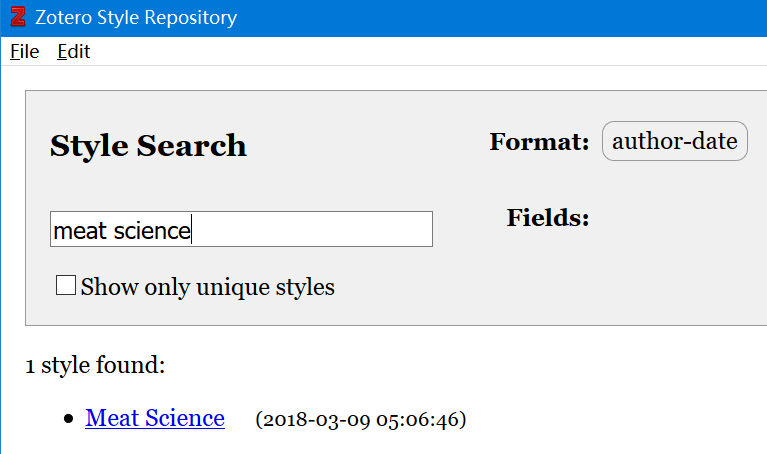
\includegraphics[width=0.7\linewidth]{ch2ZoteroStyle}
				\caption{Zotero Style仓库}
				\label{fig:ch2ZoteroStyle}
			\end{figure}
			\item
			接着会出现搜索框,可以在搜索框输入关键词,
			如文章的作者,年代,题目等,以个人经验,
			输入文章的题目搜索的结果最为准确,点击搜索结果我们希望插入的文献,
			如\autoref{fig:ch2ZoteroSearch}所示,
			然后再按回车键,则选择的文献就会插入到Word中。
			%搜索Zotero库
			\begin{figure}[htbp]
				\centering
				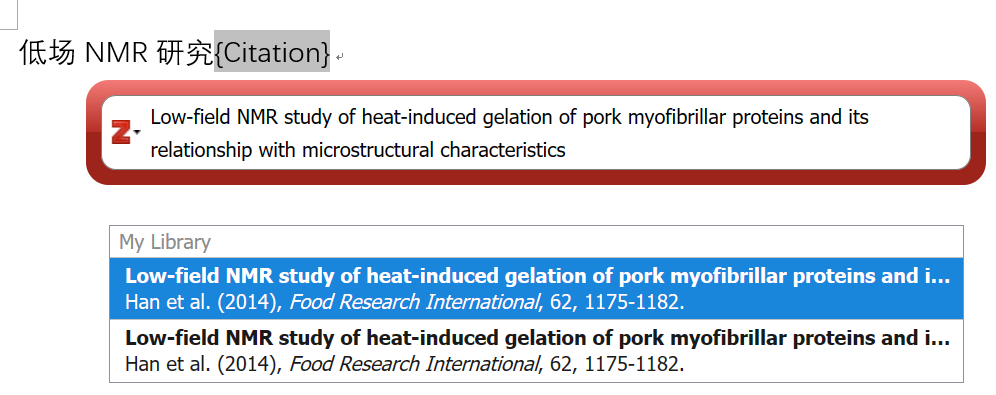
\includegraphics[scale=0.6]{ch2ZoteroSearch}
				\caption{搜索Zotero文献库}
				\label{fig:ch2ZoteroSearch}
			\end{figure}
			\item
			但参考文献现在只是插入到正文中,还没有出现文末的参考文献列表,
			要想显示它,首先将鼠标点击该Word文档的末尾,
			然后点击Zotero在Word中工具条中的第二个按钮Add/Edit Bibliography,
			刚插入的文献最会显示在文档的末尾,
			显示的格式就是我们在\autoref{fig:ch2WordInsert}选择的Style规定的格式,
			如\autoref{fig:ch2Bibliography}所示,
			仅需第一次点击这个Add/Edit Bibliography按钮,
			后面在添加、删除其他文献时,正文的引用及文末的参考文献列表最自动更新,
			是不是很方便?可以按相同的方法插入其他文献。
			
			%文末文献
			\begin{figure}[htbp]
				\centering
				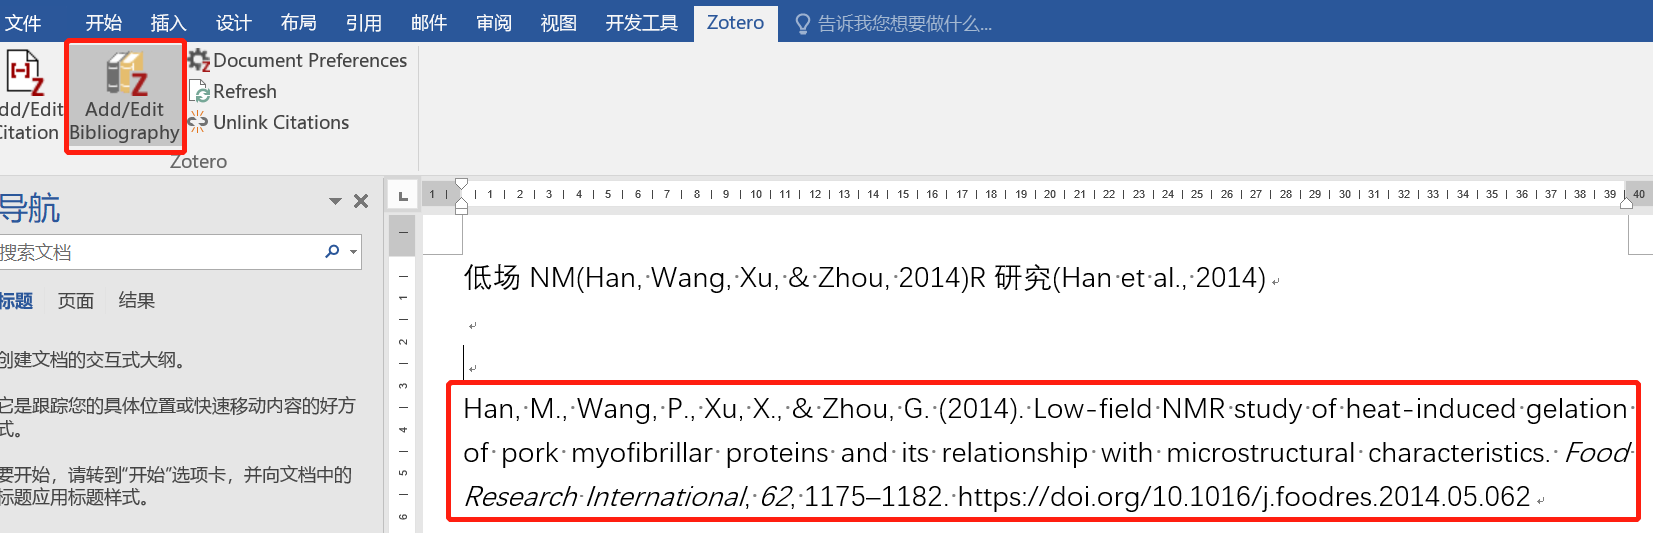
\includegraphics[scale=0.5]{ch2Bibliography}
				\caption{插入文末参考文献的方法}
				\label{fig:ch2Bibliography}
			\end{figure}
		\end{enumerate}
		\section{删除参考文献及调整参考文献的顺序}
		删除参考文献的方法比较简单,在正文中点击不需要文献,
		此时文献的背景会变为灰色,选择不需要文献,剪切或删除就可以了,
		文末的参考文献列表会自动更新。
		如果需要删除的文献的地方引用了多条文献,
		则用鼠标点击引用多条文献的地方,然后点击Zotero在Word工具条中的第一个按钮Add/Edit Citation,
		在弹出的对话框中删除不需要的文献即可,
		如\autoref{fig:ch2MultiRef}所示,当然单条参考文献的删除也可以用这个方法。
		
		调整参考文献顺序的方法是,
		将正文中的包括文献引用的部分剪切到合适的部分即可,文末的参考文献列表会自动更新,
		如果没有自动更新点击Zotero在Word工具条中Refresh按钮。
		
		%删除文献
		\begin{figure}[htbp]
			\centering
			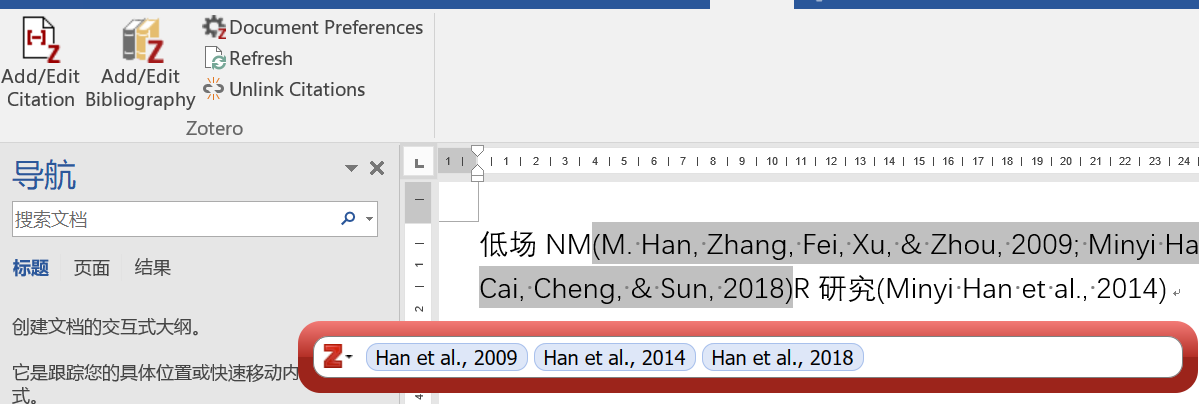
\includegraphics[width=0.7\linewidth]{ch2MultiRef}
			\caption{删除参考文献的方法}
			\label{fig:ch2MultiRef}
		\end{figure}
		\section{切换Style}\label{sec:changeStyle}
			尽管不愿意看到,但被期刊拒稿也是常见的事情,
			这时就需要修改后重新投稿,不同期刊往往正文中的引用和文末的参考文献列表格式要求不一样,
			文献重投时就需要换另外一个期刊的Style。
			换style的方法也比较简单,
			只需要点击Zotero在Word工具条中的Document Preferences按钮,
			在列表中选择合适的期刊就可以,
			如\autoref{fig:ch2ChangeStyle}所示,如果列表没有我们需要的期刊格式,
			参见\cpageref{tag:notyle}\cref{sec:insertRef}。
				%change style
				\begin{figure}
					\centering
					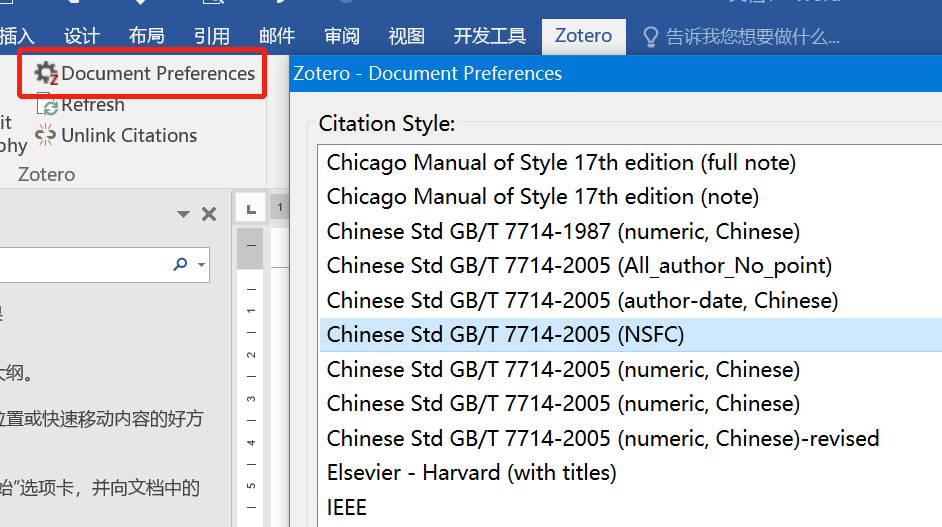
\includegraphics[width=0.7\linewidth]{ch2ChangeStyle}
					\caption{切换Style}
					\label{fig:ch2ChangeStyle}
				\end{figure}
			%zotfile install5
				\begin{figure}[htbp]
					\centering
					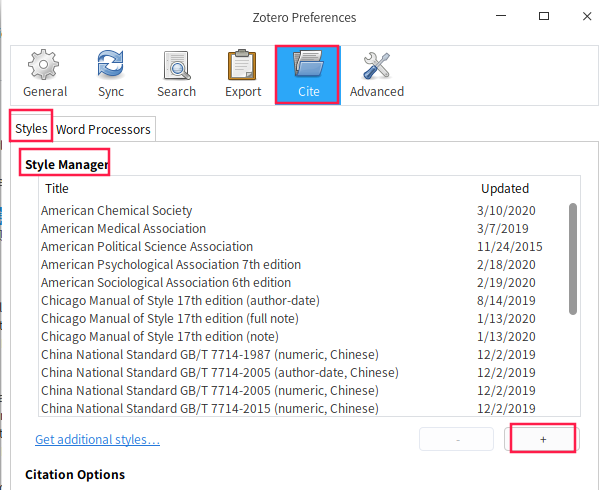
\includegraphics[scale=0.5]{ch2addStyle}
					\caption{添加本地csl文件}
					\label{fig:ch2addStyle}
				\end{figure}
		\section{添加本地csl文件}\label{sec:addStyle}
				如果Zotero仓库也没有需要的参考文献格式,则需要我们自己进行编辑Style文件,Zotero中提供了编辑Style文件的方法,
				在\url{http://editor.citationstyles.org/visualEditor/}网站上可以进行在线编辑csl文件,而后下载,同时也可以在这个网站上搜索需要的Style文件,
				可以先选择格式比较接近的期刊格式,再进行编辑。但总体上相对 Endnote的编辑格式文件而言,编辑csl文件比较复杂,如果需要可以自行百度或Google方法,或在论坛及QQ群求助。
			
				从在线编辑网站或从其他人那得到csl文件后,需要添加到本地Style目录,在格式化参考文献时才可以使用。
				添加的方法是依次点击Edit-Preferences-Cite-Styles,点击Style Mangager中右下角的“+”,如\autoref{fig:ch2addStyle}所示,找到自己的csl文件,再点击打开即可。
				%remove field codes
				\begin{figure}[htbp]
					\centering
					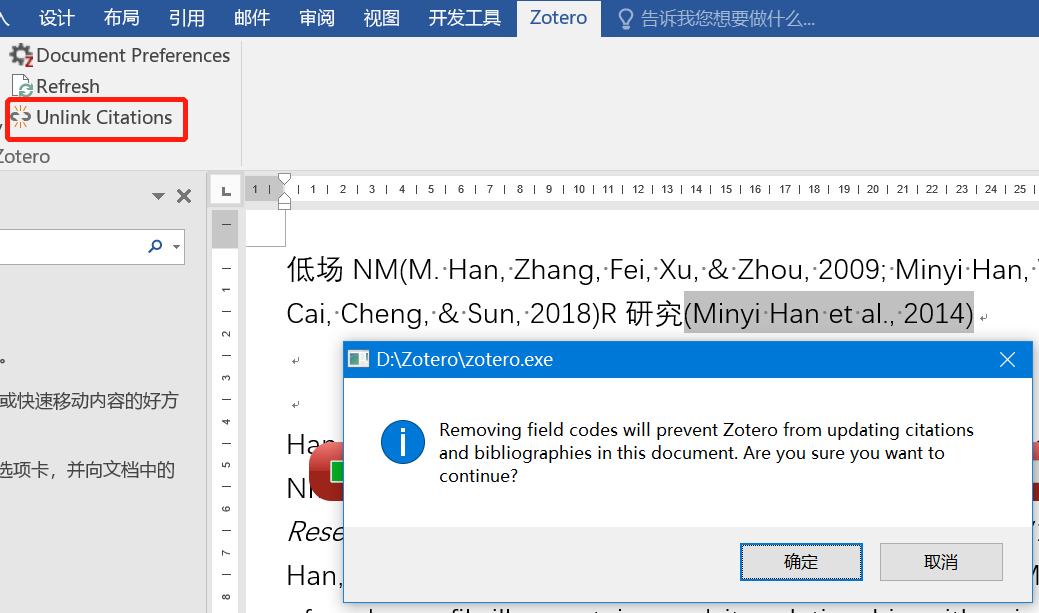
\includegraphics[scale=0.5]{ch2Unlink}
					\caption{去除域代码}
					\label{fig:ch2Unlink}
				\end{figure}
		
		\section{去除域代码}
			插入到正文的中的参考文献引用及文末的参考文献列表是以域代码的形式存在于Word文档中的,在投稿之前可以去除这些域代码,
			去除后这些参考文献与其他正文显示就没有区别了,去除的方法是,首先将文件另存一个其它文件作为备份,然后点击Zotero在Word工具条中的Unlink Citations,再点击确定,
			如\autoref{fig:ch2Unlink}所示。需要注意的是去除域代码后,再插入或删除参考文献列表就不会再自动更新了,而且再用Zotero插入的文献会自动重新编号,要想在原来基础上更新,
			只能在还保留域代码的文件中进行操作。
			
	\chapter[利用坚果云同步全文]{利用坚果云同步全文\footnote{如果没有在不同电脑同步题录和全文的需要,本章可以略过}}\label{ch:syn}		
		需要在不同电脑上阅读文献及写作的人有同步的需要。另外,如果出于对题录信息和全文备份的需要,也可以使用同步。在本章我们使用Zotero来同步题录信息,使用坚果云来同步全文信息。
			\section{注册Zotero用户}\label{sec:zotReg}
		使用Zotero来同步题录信息需要注册Zotero用户,注册的网址是\url{https://www.zotero.org/user/register},注册的流程与一般网站注册用户差别不大,
		填入用户名,Email,密码等,然后点击进行人机身份验证前的方框,根据提示完成后续步骤,最后点击 Register完成注册,
		如\autoref{fig:ch3Register}所示。注册完成后网站提示:Thanks for registering. We’ve sent an email to activate your account.
		而后查收邮箱,会收到如下内容的邮件:Thanks for signing up for a zotero.org account! Please confirm your email address 
		by clicking on the following link or pasting it into your browser: 
		\url{https://www.zotero.org/user/validate/1ab18fc52bb2b7ba6ddb},validate后面的内容会有差异,
		将这些地址复制到浏览器地址栏,按回车,如果页面显示:Success! You registered your Zotero account!则邮箱验证成功。
		如果收件箱内没有收到邮件,可以到垃圾邮件内找找,有可能这封邮件被邮件系统误认为是垃圾邮件了。不进行激活可以使用,
		但是无法创建群组(创建群组见\cref{sec:CreatGroup})。值得注意的是,注册Zotero用户时需要翻墙,
		因为这个网站需要调用Google的人机身份验证,如果不翻墙的话,无法完成注册,当然也可以请国外的亲朋好友帮忙注册用户。
		完成Zotero用户注册以后还需要在Zotero登录才能进行题录信息的同步,登录的方法见\cref{sec:syn}。
		%register zotero
		\begin{figure}[htbp]
			\centering
			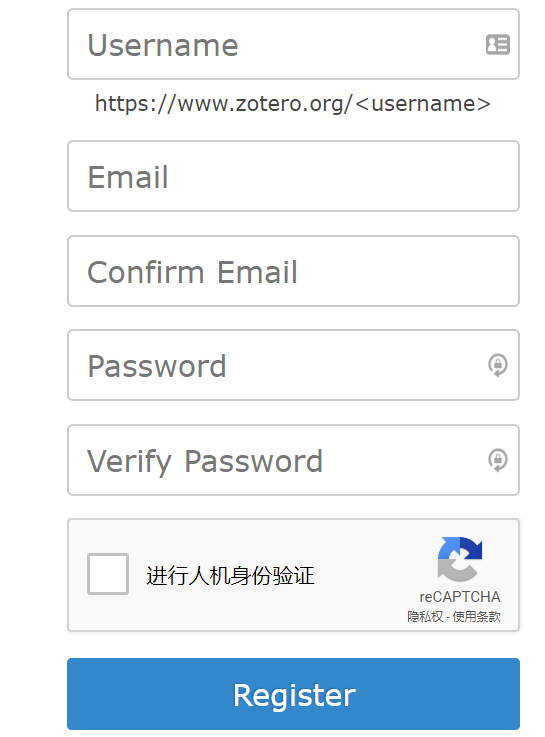
\includegraphics[width=0.3\linewidth]{ch3Register}
			\caption{注册Zotero界面}
			\label{fig:ch3Register}
		\end{figure}
		
		\section{坚果云注册及设置}\label{sec:jianguoReg}
		注册坚果云的目的主要是为了同步全文,Zotero也提供了同步全文的空间,免费的空间只有300M,2G空间的年使用费为20\$,
		如果是土豪可以选择使用Zotero来同步全文,也算是为开源社区做点贡献,支持Zotero的发展。
		另外一个可供选择的方法是使用Zotero来同步题录(Zotero提供的同步题录的空间貌似是无限的),
		而使用同步盘来同步全文,可以使用国外的\href{https://office.live.com/start/OneDrive.aspx}{OneDrive}、
		\href{https://www.dropbox.com/}{Dropbox}、
		\href{https://www.google.com/drive/}{Google Drive}、\href{https://mega.nz/}{MEGASync}等同步盘来完成,
		但这些同步盘(网盘)要么在国内无法访问,要么速度比较慢,所以我们只能选择国内的同步盘来完成。 
		这里推荐使用坚果云同步盘,这个同步盘也支持多个操作系统,它可以还提供WebDAV的方式进行访问,对于普通用户,
		它提供每个月1G的上传流量,3G的下载流量,超过以后停止上传或下载,到下个月后自动恢复,这些流量对于一般的用户也足够了。
		\begin{enumerate}
			\item 根据自己的操作系统到\url{https://www.jianguoyun.com/s/downloads}下载相应的客户端,并进行安装,
			安装过程与其他程序大同小异,在此不再赘述。安装完成以后,在系统托盘中会出现一个坚果的图标。
			如果没有图标,可以到坚果云的安装目录中双击Nutstore.exe运行坚果云同步盘,运行后需要注册一个坚果云的用户,
			如\autoref{fig:ch3JianguoRe}所示,填入需要Email、密码及昵称等信息,如\autoref{fig:ch3JianguoReg2}所示,
			点击下一步,设置需要同步的文献贮存的地址,如\autoref{fig:ch3JianguoReg3}所示,然后关闭此窗口或点击“我已知道如何使用”。
			当然也可以在坚果云的网站\url{https://www.jianguoyun.com/d/signup}上注册用户,然后在\autoref{fig:ch3JianguoRe}点击登录即可。
			
			%Jianguo reg
			\begin{figure}[htbp]
				\centering
				\begin{minipage}[t]{\dimexpr0.5\textwidth-4em}
					\centering
					
\includegraphics[scale=0.5]{ch3JianguoRe}
					\caption{坚果云用户注册步骤1}
					\label{fig:ch3JianguoRe}
				\end{minipage}
				%\hspace{1cm}
				%Jianguo reg2
				\centering
				\begin{minipage}[t]{\dimexpr0.5\textwidth-4em}
					\centering
					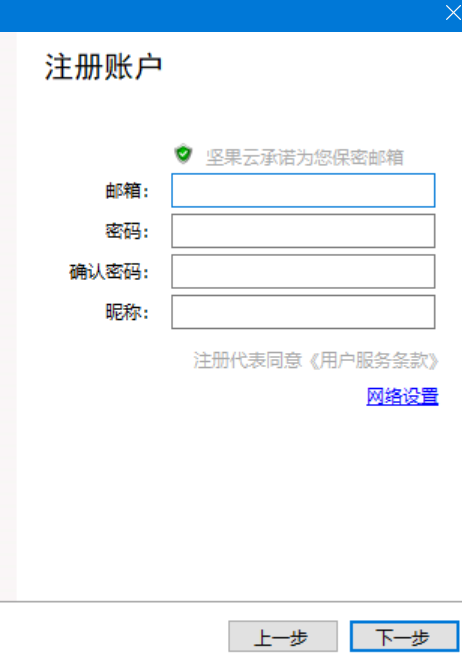
\includegraphics[scale=0.5]{ch3JianguoReg2}
					\caption{坚果云用户注册步骤2}
					\label{fig:ch3JianguoReg2}
				\end{minipage}	
			\end{figure}
			

			
			\item 此时,将文件或文件夹复制到\autoref{fig:ch3JianguoReg3}的所设置的文件内,坚果云就会将文件同步到坚果云的服务器上,
			如果在其他电脑上登录坚果云的同一用户客户端后,坚果云会自动将这些文件或文件夹同步到本地。
				%Jianguo reg3
				\begin{figure}
					\centering
					\begin{minipage}[t]{\dimexpr0.5\textwidth-4em}
					\centering
					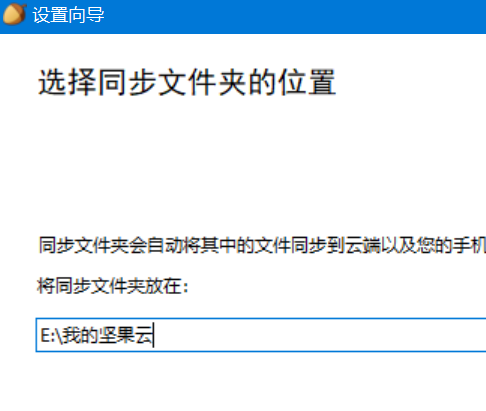
\includegraphics[scale=0.5]{ch3JianguoReg3}
					\caption{坚果云用户注册步骤3}
					\label{fig:ch3JianguoReg3}
				\end{minipage}
				%Jianguosyn folder
					\begin{minipage}[t]{\dimexpr0.5\textwidth-4em}
						\centering
						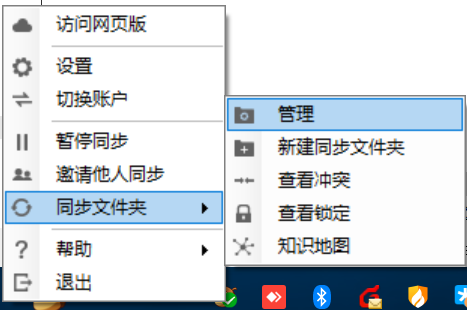
\includegraphics[width=0.5\linewidth]{ch3SynFolder}
						\caption{管理坚果云同步文件夹}
						\label{fig:ch3SynFolder}
					\end{minipage}
				\end{figure}
			\item  因为同步文献全文的需要,我们需要将同步的文件夹设置我们在\autoref{fig:ch3BaseDir}中设置的附件存放的位置,
			即图中Base directory的路径,在系统托盘中的坚果云图标上右击,然后选择同步文件夹-管理,对同步的文件夹进行重新设置,
			如\autoref{fig:ch3SynFolder}所示。
			
			\item 在弹出的对话框中,点击“移动”,然后输入或点击“浏览”找到全文附件所在的目录,值得注意的是,在用“浏览”找到文件夹,
			坚果云会自动在末尾加上“我的坚果云”,注意删除。接着坚果云会提示,文件夹已经存在,点击“合并”即可,
			如\autoref{fig:ch3JianguoMergeFolder}所示。
			%Jianguosyn change folder
			\begin{figure}[htbp]
				\centering
				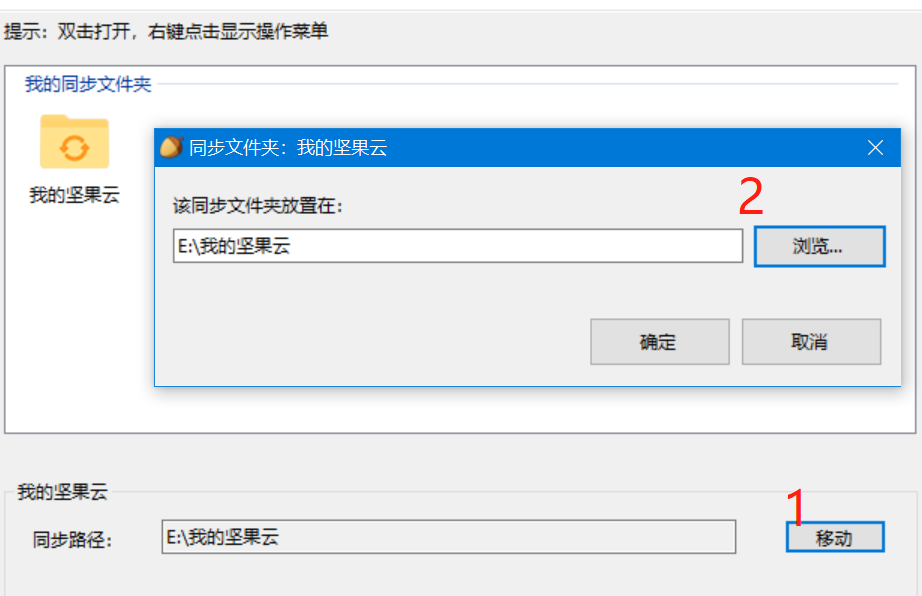
\includegraphics[scale=0.6]{ch3JianguoMoveFolder}
				\caption{更改坚果云同步文件夹}
				\label{fig:ch3JianguoMoveFolder}
			\end{figure}
			
			%Jianguosyn change folder
			\begin{figure}[htbp]
				\centering
				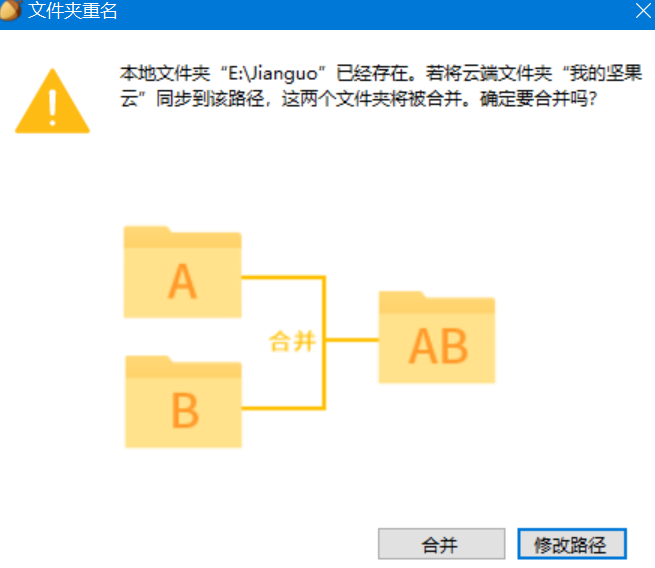
\includegraphics[width=0.5\linewidth]{ch3JianguoMergeFolder}
				\caption{合并坚果云同步文件夹}
				\label{fig:ch3JianguoMergeFolder}
			\end{figure}
		\end{enumerate}
		
		坚果云的其他问题可以访问\url{http://help.jianguoyun.com/}查找解决方法。
		
		\section{ ZotFile插件安装}\label{sec:ZotFileInstall}
		Zotero可以对题录的全文进行管理,在链接上全文以后,Zotero会将全文复制到其数据目录(数据目录在\cref{sec:newLibrary}提到)
		的storage文件夹下的一些名字比较奇怪的文件夹下,对于全文的查找和管理带来不便,因此推荐使用ZotFile插件来进行管理。
		\begin{enumerate}
			\item 到ZotFile的GitHub网站\url{https://github.com/jlegewie/zotfile/releases}
			下载ZotFile插件最新版zotfile-v.v.v-fx.xpi(v为具体的版本号),如\autoref{fig:ch3ZotFileDown}所示,
			%zotfile download
			\begin{figure}
				\centering
				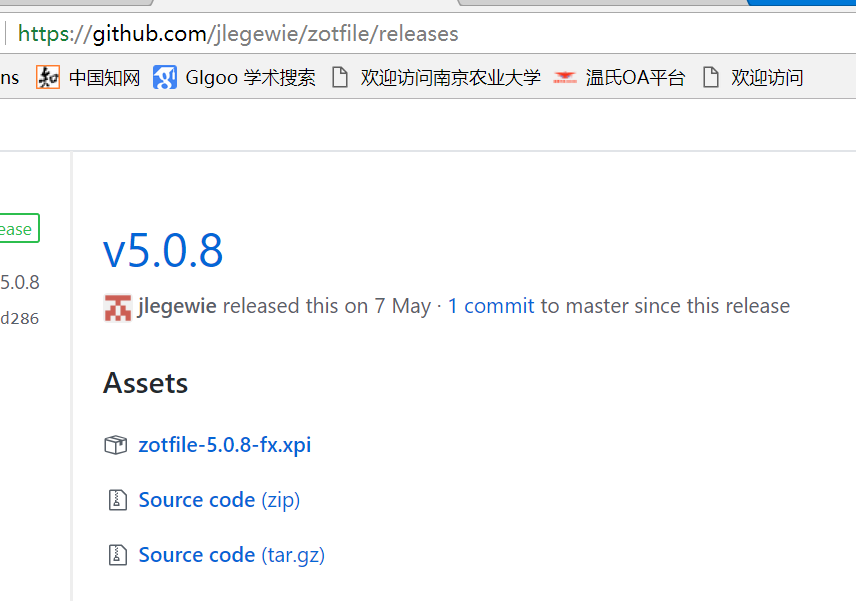
\includegraphics[scale=0.6]{ch3ZotFileDown}
				\caption{下载ZotFile插件}
				\label{fig:ch3ZotFileDown}
			\end{figure}
			
			\item
			Zotero插件与Zotero中其他插件(扩展)的安装方法相同,方法是在Zotero菜单中点击Tools-Add-ons,
			如\autoref{fig:ch3ZotFileInstall1}所示。
			%zotfile install
			\begin{figure}[htbp]
				\centering
				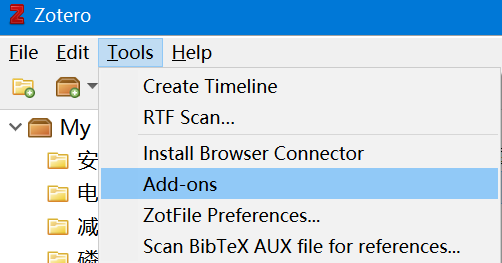
\includegraphics[width=0.5\linewidth]{ch3ZotFileInstall1}
				\caption{ZotFile插件安装步骤1}
				\label{fig:ch3ZotFileInstall1}
			\end{figure}
			\item
			在弹出的对话框中,依次点击齿轮图标-Install Add-on From File...,如\autoref{fig:ch3ZotFileInstall2}所示。
			\item
			然后找到以前下载的zotfile-v.v.v-fx.xpi(v为具体的版本号),如\autoref{fig:ch3ZotFileInstall3}所示。
			%zotfile install2-3
			
			\begin{figure}[htbp]
				\begin{minipage}[t]{0.6\linewidth}
					\centering
					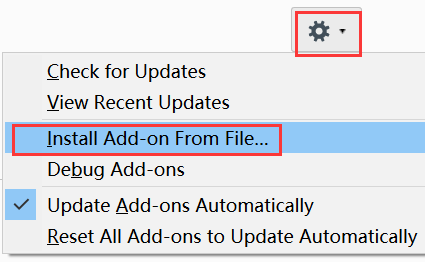
\includegraphics[width=0.7\linewidth]{ch3ZotFileInstall2}
					\caption{ZotFile插件安装步骤2}
					\label{fig:ch3ZotFileInstall2}
				\end{minipage}
				\begin{minipage}[t]{0.3\linewidth}
					\centering
					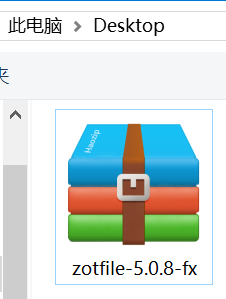
\includegraphics[width=0.6\linewidth]{ch3ZotFileInstall3}
					\caption{ZotFile插件安装步骤3}
					\label{fig:ch3ZotFileInstall3}
				\end{minipage}
			\end{figure}
			\item
			随后会出现一个3s倒计时,提示安装信任的扩展,倒计时结束后,点击Install Now开始安装,如\autoref{fig:ch3ZotFileInstall4}所示。
			\item
			安装完成后,Zotero会提示ZotFile在重启Zotero后安装,点击Restart now重启,如\autoref{fig:ch3ZotFileInstall5}所示,
			或是再安装完其他插件后一块重启,重启后会如果发现Zotero Tools-菜单下有ZoteFile Preferences...,说明ZotFile插件安装成功,
			ZotFile插件的设置见\cref{sec:zotFilePre}。
			%zotfile install4
			\begin{figure}[htbp]
				\centering
				\includegraphics[scale=0.5]{ch3ZotFileInstall4}
				\caption{ZotFile插件安装步骤4}
				\label{fig:ch3ZotFileInstall4}
			\end{figure}
			
			%zotfile install5
			\begin{figure}[htbp]
				\centering
				\includegraphics[scale=0.5]{ch3ZotFileInstall5}
				\caption{ZotFile插件安装步骤5}
				\label{fig:ch3ZotFileInstall5}
			\end{figure}
		\end{enumerate}
		
		\section{Zotero中同步设置}\label{sec:syn}
		Zotero中的同步设置包括题录同步和全文同步,我们使用Zotero提供的帐号进行题录同步,利用坚果云进行全文同步。
		
		\begin{enumerate}
			\item 
			在需要同步的电脑Zotero中依次点击Edit-Preferences,如\autoref{fig:ch3ZoteroPre1}所示。
			\item
			在弹出的Zotero Preferences对话框中点击Sync,然后在Setting中输入\cref{sec:zotReg}中申请的Zotero的用户名和密码后,
			再点击Set Up Syncing,如\autoref{fig:ch3ZoteroPre2}所示。
			%zotfile install2-3
				\begin{figure}[t]
					\centering
					\begin{minipage}[t]{\dimexpr0.5\textwidth-4em}
						\centering
						\includegraphics[scale=0.53]{ch3ZoteroPre1}
						\caption{打开Zotero设置}
						\label{fig:ch3ZoteroPre1}
				\end{minipage}
				\begin{minipage}[t]{\dimexpr0.5\textwidth-4em}
					\centering
					\includegraphics[scale=0.5]{ch3ZoteroPre2}
					\caption{Zotero同步设置}
					\label{fig:ch3ZoteroPre2}
				\end{minipage}
			\end{figure}
			\item
			如果输入的用户名、密码正确,且网络畅通,则会弹出文件同步的一些选项,注意不要选择Sync full-tex content(同步全文内容)
			和File Syncing(文件同步)前面的选项,如\autoref{fig:ch3ZoteroPre3}所示,因为Zotero提供的全文同步空间有限,
			我们在\cref{sec:jianguoReg}中设置了用坚果云同步全文,但此时Zotero还不能同步全文到其他电脑,
			还需要使用ZotFile插件将全文附件自动复制到坚果云的同步盘中。
			\item				  	
			也可以利用坚果云提供的WebDAV服务同步全文,设置方法见坚果云帮助\url{http://help.jianguoyun.com/?p=3168},
			简书文章\url{https://www.jianshu.com/p/e7f5c3e95cf4}。			  
			%zotfile install5
			\begin{figure}[htbp]
				\centering
				\includegraphics[scale=0.5]{ch3ZoteroPre3}
				\caption{Zotero同步设置}
				\label{fig:ch3ZoteroPre3}
			\end{figure}
		\end{enumerate}
		
		
		
		\section{ZotFile插件设置及将附件转移到坚果云同步盘}\label{sec:zotFilePre}
		前面提到,默认情况下Zotero将文献全文等附件会转移到数据目录中的storage下的奇怪字符的文件夹下,
		要想将文件保存到自定义的文件夹中并且用Zotero可以方便地打开,需要使用ZotFile插件来完成这项工作,
		ZotFile插件的安装见\cref{sec:ZotFileInstall}。
		\begin{enumerate}
			\item 在Zotero中依次点击Tools-ZotFile Preferences,如\autoref{fig:ch3ZotFilePre1}所示。
			%zotfile install5
			\begin{figure}[t]
				\centering
				\includegraphics[scale=0.5]{ch3ZotFilePre1}
				\caption{打开ZotFile设置}
				\label{fig:ch3ZotFilePre1}
			\end{figure}
			\item 在弹出的对话框中点击General Settings,然后点击Location of Files中Custom Location小圆圈,再点击后面的Choose,
			选择坚果云同步目录(也是全文附件的存放目录),如\autoref{fig:ch3ZotFilePre2}所示。
			%zotfile install5
			\begin{figure}[htbp]
				\centering
				\includegraphics[scale=0.7]{ch3ZotFilePre2}
				\caption{ZotFile文件夹设置}
				\label{fig:ch3ZotFilePre2}
			\end{figure}
			\item 最后,对于文献库中存在的并且已经链接全文的题录,需要用ZotFile插件重新命名附件,不同电脑之间才会同步。
			在Zotero主界面中,用鼠标或按Ctrl+A选中所有题录,然后右击依次点击Manage Attachment-Rename Attachments,
			ZotFile会弹出提示:是否移动且重命名附件,点击OK,如\autoref{fig:ch3ZotFileRename1}所示;
			ZotFile插件会根据默认的规则对附件进行重命名,并且剪切到以前设置的坚果云同步盘中,
			而且在Zotero会形成软链接,如\autoref{fig:ch3ZotFileRename2}所示,
			完成此步骤后,坚果云就会将这些附件同步附件到服务器,在其他电脑会从服务器同步到本地。
			重命名这个步骤只需要对于已经存在于文献库中并且已经链接了全文的题录(见\cref{sec:linkFulltex})进行此操作,
			对于以后从网站下载题录时同时自动下载的附件和手动添加全文的题录ZotFile会自动进行重命名并且移动到坚果云同步目录
			\footnote{在需要同步的电脑都装上坚果云、ZotFile插件并按上述设置后应该就可以在不同电脑间进行同步了。}。
			
			%zotfile rename
			\begin{figure}[htbp]
				\centering
				\includegraphics[width=0.6\linewidth]{ch3ZotFileRename1}
				\caption{ZotFile重命名附件提示}
				\label{fig:ch3ZotFileRename1}
			\end{figure}
			%zotfile rename
			\begin{figure}[htbp]
				\centering
				\includegraphics[scale=0.5]{ch3ZotFileRename2}
				\caption{ZotFile重命名附件}
				\label{fig:ch3ZotFileRename2}
			\end{figure}
		\end{enumerate}


  \chapter[Zotero群组的使用]{Zotero群组的使用\footnote{如果没有使用群组的需要,本章可以略过}}\label{ch:group}
同事之间,同一个课题组之间共享题录信息可以通过Zotero提供的群组功能实现。
我们可以创建群组并邀请其他人加入(\cref{sec:CreatGroup})。
也可以作为成员申请加入其他的群组(\cref{sec:joinGroup})。
将自己的文献复制到群组,也可以将群组文献复制到我们自己的库中(\cref{sec:copyGroupLibrary})。
   
\section{创建群组并邀请其他人加入}\label{sec:CreatGroup}
\begin{enumerate}
	\item    将\cref{sec:zotReg}申请的用户名(或Email)和密码填写到\url{https://www.zotero.org/user/login/}中,
	然后点击Login to Zotero,如\autoref{fig:ch4ZotLogin}所示\label{page:zoteroLogin}。
	%zotero login
		\begin{figure}[htbp]
			\centering\
			\begin{minipage}[t]{0.6\linewidth}
				\centering
				\includegraphics[width=0.5\linewidth]{ch4ZotLogin}
				\caption{登录Zotero网站}
				\label{fig:ch4ZotLogin}
			\end{minipage}
			%zotero group
			\centering\
			\begin{minipage}[t]{0.3\linewidth}
				\centering
				\includegraphics[width=1\linewidth]{ch4ZotGroupCreat1}
				\caption{创建群组}
				\label{fig:ch4ZotGroupCreat1}
			\end{minipage}
		\end{figure}
	
	\item 在打开的网页中,依次点击Groups-Creat a New Group,如\autoref{fig:ch4ZotGroupCreat1}所示,
	如果申请的用户名(邮箱)没有进行激活验证,则无法创建群组,激活验证的方法见\cref{sec:zotReg}。
	
	\item 在接下来打开的页面中,输入群组的名称,当群组名称下面提示的颜色变化绿色时,这个名称才可以使用。然
	后选择群组的类型:公共开放成员型(任何人可以查看和即时加入)、公共关闭会员型(任何人可以查看但用户必须申请或邀请)
	以及私秘成员型(仅成员可以查看群组,成员必须申请或被邀请),一般我们选择第二种或第三种,
	然后点击Creat Group,如\autoref{fig:ch4ZotGroupName}所示。
	%zotero group
	\begin{figure}[htbp]
		\centering
		\includegraphics[scale=0.6]{ch4ZotGroupName}
		\caption{输入群组的名称且选择群组的类型}
		\label{fig:ch4ZotGroupName}
	\end{figure}
	\item 接下来的页面中是群组的一些设置,如群组的类型,哪些人可以读群组文献库,哪些人可以对群组编辑
	,哪些人可以编辑群组文件等,根据需要进行选择即可,完成后点击Save Settings,
	如\autoref{fig:ch4ZotGroupSetting}所示,而后网页提示Group Settings Saved(群组设置已保存)。
	%zotero group
	\begin{figure}[htbp]
		\centering
		\includegraphics[width=0.3\linewidth]{ch4ZotGroupSetting}
		\caption{群组信息设置}
		\label{fig:ch4ZotGroupSetting}
	\end{figure}
	\item 群组设置完成后,点击页面顶部的Groups,在打开的页面中点击Manage Members链接来管理群组成员,
	如\autoref{fig:ch4ZotGroupInvite1}所示。在这个页面中也可以点击Manage Profile
	或Manage Library对群组的相关设置进行调整。
	%zotero group
	\begin{figure}[htbp]
		\centering
		\begin{minipage}[t]{\dimexpr.5\textwidth-1em}
			\centering
			\includegraphics[scale=0.7]{ch4ZotGroupInvite1}
			\caption{群组成员设置}
			\label{fig:ch4ZotGroupInvite1}
		\end{minipage}
		\begin{minipage}[t]{\dimexpr.5\textwidth-1em}
			\centering
			\includegraphics[scale=.6]{ch4ZotGroupInvite2}
			\caption{邀请群组成员}
			\label{fig:ch4ZotGroupInvite2}	
		\end{minipage}	 
	\end{figure}
	\item 在打开的页面中,点击Send More Invitations来发送邀请,如\autoref{fig:ch4ZotGroupInvite2}所示,
	在打开的页面的输入框中输入被邀请人的用户名或Email地址,多个用户之间用英文逗号间隔,
	然后再点击Invite Members,如\autoref{fig:ch4ZotGroupInvite3}所示,
	而后会返回邀请的结果,\autoref{fig:ch4ZotGroupInvite4}。
	%Group Invite Member2
	\begin{figure}[t]
		\begin{minipage}[b]{\dimexpr.5\textwidth-1em}
			\centering
			\includegraphics[scale=1]{ch4ZotGroupInvite3}
			\caption{发送邀请}
			\label{fig:ch4ZotGroupInvite3}
		\end{minipage}
		\begin{minipage}[b]{\dimexpr.5\textwidth-1em}
			\centering
			\includegraphics[scale=1]{ch4ZotGroupInvite4}
			\caption{邀请的结果}
			\label{fig:ch4ZotGroupInvite4}
		\end{minipage}
	\end{figure}
	\item 当被邀请用户按\cpageref{page:zoteroLogin}方法登录Zotero网站,
	并点击Group后在页面右侧会显示收到的群组邀请信息,点击Join,即可加入群组,如\autoref{fig:ch4ZotGroupInvite5}所示,
	然后刷新网页后就会显示当前已经加入的群组,如\autoref{fig:ch4ZotGroupInvite6}所示。
	%Group Invite Member2
	\begin{figure}[t]
		\begin{minipage}[b]{\dimexpr.5\textwidth-1em}
			\centering
			\includegraphics[scale=.8]{ch4ZotGroupInvite5}
			\caption{点击Join加入群组}
			\label{fig:ch4ZotGroupInvite5}
		\end{minipage}
		\begin{minipage}[b]{\dimexpr.5\textwidth-1em}
			\centering
			\includegraphics[scale=.8]{ch4ZotGroupInvite6}
			\caption{刷新网页显示已经加入到群组}
			\label{fig:ch4ZotGroupInvite6}
		\end{minipage}
	\end{figure}
	\item 按\cref{sec:syn}的描述,用自己的用户名密码在Zotero登录后,
	在Zotero左侧面板会也会显示已经加入的群组,如\autoref{fig:ch4ZotGroupInvite7}所示,
	而且会自动将群组中的文献同步到本地。
	%Joined zotero group 
	\begin{figure}[t]
			\begin{minipage}[b]{\dimexpr.5\textwidth-1em}
				\centering
				\includegraphics[scale=.8]{ch4ZotGroupInvite7}
				\caption{登录Zotero后也可以显示已经加入的群组}
				\label{fig:ch4ZotGroupInvite7}
			\end{minipage}
			\begin{minipage}[b]{\dimexpr.5\textwidth-1em}
				\centering
				\includegraphics[scale=.8]{ch4ZotSearchGroup1}
				\caption{搜索群组}
				\label{fig:ch4ZotSearchGroup1}
			\end{minipage}
	\end{figure}
	
\end{enumerate}

\section{申请加入群组}\label{sec:joinGroup}
\begin{enumerate}
	\item 按\cpageref{page:zoteroLogin}所示方法,用自己的用户名/Email地址和密码登录\url{https://www.zotero.org/user/login/}网站。
	\item 登录网站后依次点击Groups-Search for Groups,如\autoref{fig:ch4ZotSearchGroup1}所示。
	\item 在打开的网页中点击Groups,然后在框中输入群组的名称,点击Search Groups,如\autoref{fig:ch4ZotSearchGroup2}所示。
	
	
	%Join zotero group 
	\begin{figure}[t]
		\begin{minipage}[b]{\dimexpr.3\textwidth-1em}
			\centering
			\includegraphics[scale=.5]{ch4ZotSearchGroup2}
			\caption{输入搜索的群组名称}
			\label{fig:ch4ZotSearchGroup2}
		\end{minipage}
		\begin{minipage}[b]{\dimexpr.3\textwidth-1em}
			\centering
			\includegraphics[scale=0.5]{ch4ZotSearchGroup3}
			\caption{群组搜索结果}
			\label{fig:ch4ZotSearchGroup3}
		\end{minipage}
		\begin{minipage}[b]{\dimexpr.4\textwidth-1em}
			\centering
			\includegraphics[scale=0.5]{ch4ZotSearchGroup4}
			\caption{点击Join申请加入群组}
			\label{fig:ch4ZotSearchGroup4}
		\end{minipage}
	
	\end{figure}
	\item 在搜索结果中点击需要申请加入的群组名称,如\autoref{fig:ch4ZotSearchGroup3}所示,
	然后在打开页面的右侧点击Join申请加入群组,如\autoref{fig:ch4ZotSearchGroup4},
	然后网页会提示:You have applied to join this group. A group admin must approve your application.
	%zotero group
		\begin{figure}[htbp]
			\centering\
			\begin{minipage}[t]{0.6\linewidth}
				\centering
				\includegraphics[scale=0.8]{ch4ZotSearchGroup5}
				\caption{管理员批准加入群组申请}
				\label{fig:ch4ZotSearchGroup5}
			\end{minipage}
			%
			\begin{minipage}[t]{0.3\linewidth}
				\centering
				\includegraphics[scale=.9]{ch4ZotGroupNewColl}
				\caption{在群组中新建分类的结果}
				\label{fig:ch4ZotGroupNewColl}
			\end{minipage}
		\end{figure}

	\item 管理员的邮箱中会收到Zotero发送的邮件,提示有人申请加入群组,此邮件也有可能被邮箱系统放入到垃圾邮件中。
	群组管理员根据邮件提示登录到Zotero网站,点击Approve即可,如\autoref{fig:ch4ZotSearchGroup5}所示。

\end{enumerate}

\section{群组文献添加和复制}\label{sec:copyGroupLibrary}
\begin{enumerate}
	\item 在群组库中,也可以像\cref{sec:newLibrary}描述的那样通过File-New Collection...或右击群组的名称选择New Collection...
	建立分类及子分类以方便题录的管理,建立分类的结果如\autoref{fig:ch4ZotGroupNewColl}所示。
	\item 添加群组文献实现可以通过两种方法实现,一是直接将Zotero左侧面板自己文献库中的题注拖放到群组库的相应文件夹中,
	如\autoref{fig:ch4ZotGroupDragCitation}所示。
	另外,也可以在选中群组库文件夹后,通过\cref{sec:ImportFromWeb}$\sim$\cref{sec:ManualImport}的方法在线导入或手动输入题录。
	%drag citataion
		\begin{figure}[htbp]
			\centering
			\includegraphics[scale=0.9]{ch4ZotGroupDragCitation}
			\caption{通过拖放的方式在群组库中添加文献}
			\label{fig:ch4ZotGroupDragCitation}
		\end{figure}

		%drag citataion
			\begin{figure}[htbp]
			\centering
			\includegraphics[scale=0.9]{ch4ZotGroupDrayFromGroup}
			\caption{通过拖放的方式复制群组库文献到本地}
			\label{fig:ch4ZotGroupDrayFromGroup}
			\end{figure}
		\item 看到群组库中有我们感兴趣的文献后,我们可以将文献复制到自己文件夹中,
		复制的方式是在群组库选中需要的文献,拖放到本地库的相应文件夹中即可,
		如所示\autoref{fig:ch4ZotGroupDrayFromGroup}。
	\end{enumerate}

%第五章
  \chapter{高级应用及疑难解答}\label{ch:questions}
	本章讲述了一些高级问题讨论和疑难解答,
	Zotero 标签的使用 \cref{sec:tag};在CNKI在导入题录的同时也下载全文(\cref{sec:cnki_fulltext});
	在撰写中文文章时,参考文献列表中中文作者后面为“等”,英文为“et al”(\cref{sec:etal});
	文献题目中的格式(斜体、上标、下标、大小写,\cref{sec:italic},\cref{sec:case})等问题。
		

	\section{Zotero 标签的使用} \label{sec:tag}
			在默认设置情况下,Zotero界面左下角的区域显示的是Zotero的标签,
			我们可以使用Zotero的文件夹(创建文件夹的操作见\cref{sec:newLibrary})和标签功能来管理文献,
			一般情况下,我们按不同的专题或研究方向将文献放到不同的文件夹,这样管理起来比较方便。
			既然有了文件夹为什么还需要使用标签呢?因为有时候,一篇文献可能属于多个文件夹,
			例如我们可以将所有文献分为“已读”和“未读”两类;或是挂个某个项目编号的文章也可能属于多个文件夹。
			当然这种情况下,也可以把文献复制到不同的文件夹或是建立子文件夹(再建立“已读”和“未读”子文件夹),
			但操作起来会比较麻烦。这时候就可以使用Zotero的标签功能,实现这种文献的“交叉”管理
			\footnote{除了标签之外,可以通过
		分类(文件夹)和关联对文献进行管理,详见
		\href{https://zhuanlan.zhihu.com/p/275707703}{Zotero分类、标签和关联的使用。}}。
			
			Zotero在导入文献时,会将文献的关键词以及主题作为标签导入到文献库中(称为“自动标签”),
			看起来比较杂乱,我们可以使它不显示,或是删除自动生成的这些标签。方法是点击标签管理区域的彩色块位置
			,点击Show Automatic前的方框,使之不选中如\autoref{ch5DeleteAutoTag}所示。
			或是点击Delete Automatic Tags in This Library...,在弹出的对话框中点击OK,
			即会删除自动标签,如\autoref{ch5DeleteAutoTagOK}所示。也可以在标签上右击,再点击Delete Tag...,
			删除单个标签。
			
				\begin{figure}[htbp]
					\centering
					\includegraphics[scale=0.8]{ch5DeleteAutoTag}
					\caption{使自动标签不显示或删除自动标签}
					\label{ch5DeleteAutoTag}
				\end{figure}
				\begin{figure}[htbp]
					\centering
					\includegraphics[scale=0.8]{ch5DeleteAutoTagOK}
					\caption{确认删除自动标签}
					\label{ch5DeleteAutoTagOK}
				\end{figure}
			
			我们如果使用自己的标签功能最好把这个功能禁用,方法是在Zotero中依次点击Edit-Preference-General-Miscellaneous,在界面的中间位置,在
			Automatically tag items with keywords and subject headings前面方框内点击,使它处理不选中状态,如\autoref{ch5DisableImportTag}所示。
				\begin{figure}[htbp]
					\centering
					\includegraphics[scale=0.8]{ch5DisableImportTag}
					\caption{导入文献不自动导入关键词作为标签}
					\label{ch5DisableImportTag}
				\end{figure}
						
			在Zotero中添加标签的方法是,首先选中需要添加标签的文献,在右侧Tags下点击Add,输入需要命名的标签,如\autoref{fig:ch5Add_tag}所示,这种方法适用于新建一个标签,一次只能为一篇文献添加标签,但可以为一篇文献添加多个标签,只需要不断点击Add即可,如果想删除一篇文献的标签,可以点击“-”号。也可以将多篇文献选中,然后拖动到左下角标签区域的某个标签上,这样可以为多篇文章添加标签,但前提是这个标签已经存在。
				\begin{figure}[htbp]
					\centering
					\includegraphics[scale=0.8]{ch5Add_tag}
					\caption{给一篇文献添加标签}
					\label{fig:ch5Add_tag}
				\end{figure}
			
			以后需要某个标签的文献时,只需要在标签区域点击这个标签,右侧文献显示区域就会显示这个标签下的所有文献,如\autoref{ch5Seclect_tag}所示。
				\begin{figure}[htbp]
					\centering
					\includegraphics[scale=0.8]{ch5Seclect_tag}
					\caption{点击某一标签就会显示这个标签下的文献}
					\label{ch5Seclect_tag}
				\end{figure}
			
			在Zotero的标签区域,你会发现所有的标签是按字母排列的,中文标签排在英文之后。
			我们可以给标签指定颜色,指定了颜色的标签会排到前面,比较美观。
			方法是右击需要设定颜色的标签,点击“Assign Color”,
			如\autoref{ch5Assign_color}所示,一个库中可以给9个标签指定颜色,
			在这个界面也可以给标签重命名或删除标签。
				\begin{figure}[htbp]
					\begin{minipage}[t]{\dimexpr0.5\textwidth-4em}
						\centering
						\includegraphics[scale=0.7]{ch5Assign_color}
						\caption{给标签指定颜色1}
						\label{ch5Assign_color}
					\end{minipage}
					\begin{minipage}[t]{\dimexpr0.5\textwidth-4em}
						\centering
						\includegraphics[scale=0.6]{ch5SetTagColor}
						\caption{给标签指定颜色2}
						\label{ch5SetTagColor}
					\end{minipage}
			\end{figure}	
					
					
					
				
				
在弹出的对话框中给标签指定喜欢的颜色和标签位置,
点击Set Color,如\autoref{ch5SetTagColor}所示。
				
				如果设置的标签过多,找不到需要的标签,
				可以在标签区域的最下方输入标签的名称进行搜索,
				上方会显示搜索得到的结果,如\autoref{ch5SearchTag}所示。
				\begin{figure}[htbp]
					\centering
					\includegraphics[scale=0.8]{ch5SearchTag}
					\caption{搜索标签}
					\label{ch5SearchTag}
				\end{figure}
			
		\section{更新CNKI.js,当有权限时在CNKI导入题录的同时下载全文}\label{sec:cnki_fulltext}
				一直以来,我们只能在CNKI在导入题录,而全文CAJ或PDF文件都不能同时下载下来。
				近期,有国内的网友对CNKI的translator\footnote{translator相当于一个翻译器,
				将网页上的元素翻译为在Zotero导入网页信息时可以识别的Zotero条目。}进行了修改,
				\href{https://www.linxingzhong.top/posts/2019-11-5/?tdsourcetag=s_pctim_aiomsg}{参见网址}。
				如果你当前在导入CNKI题录时不能同时下载全文,请参考下面的步骤:
			\begin{enumerate}
				\item\label{it:cnkijs}
					首先到\href{https://github.com/Zotero-CN/translators_CN}{ Zotero translators 
					中文维护小组的GitHub\footnote{在这个GitHub上除了CNKI的translator之外,
					还有其他几个国内经常使用的数据库,如万方数据、维普、百度学术、谷粉学术、
					专利搜索网站SooPAT。如果Zotero不带或使用异常,可以选择使用这个网站上的。} 
					\url{ https://github.com/Zotero-CN/translators_CN}}下载CNKI.js
					,在CNKI.js处右击,选择“链接另存为(K)...”,放到自己的位置,如\autoref{fig:ch5CNKIJS}图示:
						%CNKI.js
					\begin{figure}[htbp]
						\centering
						\includegraphics[scale=0.9]{ch5CNKIJS}
						\caption{CNKI.js下载}
						\label{fig:ch5CNKIJS}
					\end{figure}
				\item
				  将上一步下载的CNKI.js复制到Zotero的translator目录中(如\path{E:\hmy\zotero\translator})。
				  或在上一步直接将CNKI.js下载到这个目录中。覆盖原来的CNKI.js,保险起见,
				  可以先将原来的CNKI.js复制到其他地方备份,如果有问题再复制回来。
				  如果忘了自己的translator目录,可以在Zotero中依次点击Edit-Preferences-Advanced-Files and Folders
				  中查看,如\autoref{fig:ch5translatorDir}所示:
				  	%translator dir
					  \begin{figure}[htbp]
					  	\centering
					  	\includegraphics[scale=0.9]{ch5translatorDir}
					  	\caption{查看translator目录所在的文件夹}
					  	\label{fig:ch5translatorDir}
					  \end{figure}
				  \item
				  在浏览器的Zotero插件上右击,依次点击选项-Advanced-Translator下面的Update Translators,
				  见\autoref{fig:ch5ZoteroOption},\autoref{fig:ch5ZoteroUpdateTran}:
				  %Zotero选项
				  \begin{figure}[htbp]
				  	\centering
				  	\includegraphics[scale=1]{ch5ZoteroOptions}
				  	\caption{右击Zotero在浏览器中的图标}
				  	\label{fig:ch5ZoteroOption}
				  \end{figure}
			     %更新translator
			     \begin{figure}[htbp]
			  	  \centering
			  	  \includegraphics[scale=1]{ch5ZoteroUpdateTran}
			  	  \caption{更新translator}
			  	  \label{fig:ch5ZoteroUpdateTran}
			     \end{figure}
		  \item
		  登录\href{http://www.cnki.net}{CNKI},试一下在有权限情况时下载题录的同时是否把全文pdf也下载了,
		  具体方法参见\cref{sec:cnki}。如果不行,试着重新启动浏览器和Zotero,或是重启一下系统。
		   \end{enumerate}
	   
	   上面的操作步骤也可参见知乎专栏文章\href{https://zhuanlan.zhihu.com/p/90638718}{[Zotero]
	   有权限时在导入CNKI题录时同时下载全文的方法\url{https://zhuanlan.zhihu.com/p/90638718}}。
	
		\section{如何设置Zotero生成的参考文献格式,刷新后不变?}\label{sec:refresh}
		Endnote在Word的工具栏中可以设置文末参考文献列表的格式,而Zotero中没有这些功能,
		如果只是单纯设置格式,那么再插入其他或修改参考文献后格式就会恢复到默认的字体格式,
		但可以通过在Word中的“书目”样式来实现,而且刷新后也可以保持不变。
		参考 网友@滏阳河边捉蚯蚓 的方法,具体步骤如下:
			\begin{enumerate}
				\item
				用Zotero在Word中生成参考文献后(参见\cref{sec:insertRef}),
				将光标定位到参考文献中,或选中生成的参考文献,点击样式处右下角的箭头,
				然后向下拉找到“书目”,再点击“书目”后面的向下的箭头,
				点击“修改”,如\autoref{fig:ch5Biblio}所示:
		    		\begin{figure}[htbp]
			    		\centering
			    		\includegraphics[scale=0.5]{ch5Biblio}
			    		\caption{找到书目样式}
			    		\label{fig:ch5Biblio}
		    	  \end{figure}
		    	\item
				根据期刊或毕业论文排版要求设置格式,如可以将英文字体设置为Times New Roman,
				字号:五号,点击“格式”-“段落”在弹出的对话框中设置缩进,行间距等,如
				可以设置行间距为20磅,如\autoref{fig:ch5Format},\autoref{fig:ch5Hanging}所示。
			    	%样式修改
			    	\begin{figure}[t]
			    		\centering
			    		\includegraphics[scale=0.5]{ch5Format}
			    		\caption{对样式进行修改}
			    		\label{fig:ch5Format}
			    	\end{figure}
		    	 
			    	\begin{figure}[htbp]
			    		\centering
			    		\includegraphics[scale=0.5]{ch5Hanging}
			    		\caption{设置悬挂缩进}
			    		\label{fig:ch5Hanging}
			    	\end{figure}
		    	\item
				 如果都确定后,发现文末参考文献格式没有变化,那么选中所有参考文献,再点击“样式”中的“书目”,
				 如\autoref{fig:ch5FreshFinalformat}所示。
			    	\begin{figure}[htbp]
			    		\centering
			    		\includegraphics[scale=0.8]{ch5FreshFinalformat}
			    		\caption{全选后再次点击书目}
			    		\label{fig:ch5FreshFinalformat}
			    	\end{figure}
		    	\item
		    	如果再插入文献或刷新后,会发现格式仍然是我们刚才设置的格式。
		    	%\url{https://zhuanlan.zhihu.com/p/58969571}
			\end{enumerate}
		\section{中文作者后为“等”,英文为“et al”的设置方法}\label{sec:etal_set}	
			一直以来在Word中同时引用中英文文献,
			使用默认的Chinese-gb7714-1987-numeric.csl格式化文献,
			在作者超过三个后同时显示“et al”和“等”是写作的难题(latex可以轻松解决),
			解决方法或者是手动修改,或是编写宏批量替换,
			使中文的参考文献中超过3个作者显示为“等”,英文的为“et al”,见\cref{sec:etal}。
			无论哪种方式在刷新文档,插入删除文献后会恢复为不正常的情况,
			或是都显示为“等”,或显示为“et al”。


			\href{https://juris-m.github.io/release/}{JurisM}是Zotero的修改版,
			在法律文献,多语言方面进行了加强,我们可以借用\href{https://juris-m.github.io/release/}
			{JurisM}对csl的扩展,实现中文作者后为“等”,英文为“et al”。具体步骤为:
			\begin{enumerate}
				\item 到\url{https://juris-m.github.io/styles/},
				点击JM Chinese Std GB/T 7714-2005 (numeric, Chinese)前面的下载链接,
				如\autoref{fig:ch5jmStyle-down}所示:
				%下载安装JM Style
				\begin{figure}[htbp]
					\centering
					\includegraphics[scale=0.5]{ch5jmStyle-down}
					\caption{下载安装JM Style}
					\label{fig:ch5jmStyle-down}
				\end{figure}
				浏览器中会弹出是否安装Style的提示,点击OK,则会出现正在安装的提示
				如\autoref{fig:ch5ZotoerInstallStyle},\autoref{fig:ch5InstallingStyle-error1}
				所示:
				%安装style及错误提示
				\begin{figure}[htbp]
					\centering
					\begin{minipage}[t]{\dimexpr0.5\textwidth-4em}
						\centering
						\includegraphics[width=0.7\linewidth]{ch5ZotoerInstallStyle}
						\caption{是否安装的提示}
						\label{fig:ch5ZotoerInstallStyle}
					\end{minipage}
					\begin{minipage}[t]{\dimexpr0.5\textwidth-4em}
						\centering
						\includegraphics[scale=0.7]{ch5InstallingStyle-error1}
						\caption{正在安装的提示}
						\label{fig:ch5InstallingStyle-error1}
					\end{minipage}
				\end{figure}
				这个等待时间可能比较长,期刊会出现一些错误提示,
				如
				\autoref{fig:ch5InstallingStyle-error}所示,
				点击OK继续\footnote{也可以在此网页上,在链接右击,
				选择链接另存为,将Style下载下来,再进行安装,
				本地安装style的方法见\cref{sec:addStyle}。}:
				%安装style及错误提示
				\begin{figure}[htbp]
					\centering
						\includegraphics[scale=0.7]{ch5InstallingStyle-error}
						\caption{可能有错误提示,点击OK}
						\label{fig:ch5InstallingStyle-error}
					\end{figure}
			\item 在插入或格式化参考文献格式时,选择
				JM Chinese Std GB/T 7714-2005 (numeric, Chinese)这个Style,
				如\autoref{fig:ch5Jmstyle-select}所示:
				%选择JM Style
				\begin{figure}[htbp]
					\centering
					\includegraphics[scale=0.7]{ch5Jmstyle-select}
					\caption{选择JM Style}
					\label{fig:ch5Jmstyle-select}
				\end{figure}
			\item 正常情况下,中文参考文献三个作者后面应该为“等”,英文为“et al”,
			如果不正常,在Zotero库中将英文文献的“Language”字段修改为“en”
			\footnote{我遇到的不正常的情况是英文作者后面也是“等”,如果中文作者后面
			成了“et al”,可以尝试修改中文文献的“Language”字段修改为“cn”或“中文”试试。},
			如\autoref{fig:ch5JmLanguage}所示:
			%将英文文献的“Language”字段修改为“en”
			\begin{figure}[htbp]
				\centering
				\includegraphics[scale=0.7]{ch5JmLanguage}
				\caption{将英文文献的“Language”字段修改为“en”}
				\label{fig:ch5JmLanguage}
			\end{figure}
			\item 修改完毕后,返回Word,点击Zotero工具条中Refresh按钮,最终结果
			如\autoref{fig:ch5Jm-final}所示:
			%点击Refresh后最终结果
			\begin{figure}[htbp]
				\centering
				\includegraphics[scale=0.6]{ch5Jm-final}
				\caption{点击Refresh后最终结果}
				\label{fig:ch5Jm-final}
			\end{figure}
			\end{enumerate}
		
			本节文字也可见
		\href{https://zhuanlan.zhihu.com/p/317108621}
		{[Zotero]使用JurisM Style实现同时生成“et al”和“等”}
		(\url{https://zhuanlan.zhihu.com/p/317108621})。

		\section{使用宏,使中文作者后为“等”,英文为“et al”}\label{sec:etal}
			由于现在的csl不支持多语言,在用Chinese-gb7714-1987-numeric.csl、
			Chinese-gb7714-2005-numeric.csl或Chinese-gb7714-2015-numeric.csl
			生成的参考文献英文作者超过3个后面也是“等”,如\autoref{fig:ch5etal_error}所示(正确的应该是et al)。
			下面的方法可以实现将英文作者后面的“等”替换为“et al”,
			而中文作者后面保持不变(以Word 2016为例)\footnote{其他参考文献管理软件如Mendeley,
			EndNote生成的参考文献同样适合。要在最后定稿后再运行此宏,参考文献更新后需要重新运行。
			方法来源于:\href{https://zhuanlan.zhihu.com/p/53594081}
			{滏阳河边捉蚯蚓:自定义宏批量修改csl生成参考文献书目的错误。}}。
			\begin{figure}[htbp]
				\centering
				\includegraphics[scale=0.5]{ch5etal_error}
				\caption{英文三个作者以上也是“等”}
				\label{fig:ch5etal_error}
			\end{figure}
		

			\begin{enumerate}
				\item 在word 2016中依次点击开发工具-宏(如果没有开发工具,也可在视图中找到“宏”),
				在宏名下面的文本框中随便输入一个名称(如abc),点击“创建”,
				如\autoref{fig:ch5macro1}。
					\begin{figure}[htbp]
						\centering
						\includegraphics[scale=0.5]{ch5macro1}
						\caption{创建宏的步骤}
						\label{fig:ch5macro1}
					\end{figure}
				\item 将Sub abc到End Sub全部删除,用下面的代码替换,
				如\autoref{fig:ch5macro2},\autoref{fig:ch5macro3}:
				%宏代码
				\begin{lstlisting}[language=VBScript]
					Sub deng2etal()
					'
					' deng2etal macro
					' English等 -> english, et al
					'
					With Selection.Find
					.Forward = True
					.ClearFormatting
					.Text = "(<[A-z]@, )等"
					With .Replacement
					.ClearFormatting
					.Text = "\1et al"
					End With
					.Wrap = wdFindStop
					.Execute Replace:=wdReplaceAll, MatchWildcards:=True
					End With
					End Sub
			\end{lstlisting}
			
			\begin{figure}[htbp]
				\centering
				\includegraphics[scale=0.9]{ch5macro2}
				\caption{将宏替换}
				\label{fig:ch5macro2}
			\end{figure}
			\begin{figure}[htbp]
				\centering
				\includegraphics[scale=0.5]{ch5macro3}
				\caption{宏替换后的效果}
				\label{fig:ch5macro3}
			\end{figure}
		\item 然后关闭宏编辑窗口。
		\item 依次点击开发工具-宏(如果没有开发工具,也可在视图中找到“宏”),
		点击deng2etal,再点击“运行”,如\autoref{fig:ch5macro4},
		最终效果如\autoref{fig:ch5macro5}所示\footnote{
			上面的做法是将“等”用正则表达式的方法替换为“et al”,
						也可以用另外的正则表达式,将“et al”替换为“等”,
						请参见\href{https://zhuanlan.zhihu.com/p/60029219}
						{Zotero+Word2016参考文献中英文混排,解决et al和等的问题,另一思路}。
		}:
			\begin{figure}[htbp]
				\centering
				\includegraphics[scale=0.5]{ch5macro4}
				\caption{运行宏}
				\label{fig:ch5macro4}
			\end{figure}
			\begin{figure}[htbp]
				\centering
				\includegraphics[scale=0.5]{ch5macro5}
				\caption{最终效果}
				\label{fig:ch5macro5}
			\end{figure}
		\item 当然也可以为这个宏分配一个按钮,点击快速访问工具栏最后的向下箭头
		选择“其他命令(M)...”,如\autoref{fig:ch5macro6_button}所示,	
				\begin{figure}[htbp]
					\centering
					\includegraphics[scale=0.5]{ch5macro6_button}
					\caption{为宏分配按钮步骤1}
					\label{fig:ch5macro6_button}
				\end{figure}
		\item 然后在“从下列位置选择命令(C)”处点击 “宏”,找到刚才创建的宏,点击“添加”,
		再点“确定”返回,如\autoref{fig:ch5macro6_button2}所示。		
				\begin{figure}[htbp]
					\centering
					\includegraphics[scale=0.5]{ch5macro6_button2}
					\caption{为宏分配按钮步骤2}
					\label{fig:ch5macro6_button2}
				\end{figure}
		\item 在此步骤也可以为宏设置其他按钮形状,添加后,选中这个宏,再点“修改”,
		选择喜欢的按钮形状,然后点“确定”返回即可,如\autoref{fig:ch5macro6_button3}所示。
		此时快速访问工具栏上就会有这个宏的按钮了,用时点击即可。	
			\begin{figure}[htbp]
				\centering
				\includegraphics[scale=0.5]{ch5macro6_button3}
				\caption{为宏分配按钮步骤3}
				\label{fig:ch5macro6_button3}
			\end{figure}
		\end{enumerate}
			
						
			 	
		\section{author+year格式下,et al如何变为斜体?}\label{sec:etal_italic}
			变为斜体的地方两个,一个是文中的引文部分(Inline Citations),
			另一个是文末的参考文献列表部分(Bibliography)。
			主要是通过修改style即csl文件实现的。修改csl文件可以通过Zotero
			自带的Style Editor来完成(在Zotero中,
			依次点击Edit-Preferences-Cite-Styles,在Style Mangager选
			中要修改的Style再点击Tools下面的Style Editor按钮),
			但这种方法需要对csl语言比较熟悉。
			另一种方法是通过csl文件在线编辑方式进行,操作比较直观。
			下面以springer-basic-author-date 这种格式的csl进行修改。	
			\begin{enumerate}
				\item 
				在浏览器地址栏中输入
				\href{https://editor.citationstyles.org/searchByName/}
				{https://editor.citationstyles.org/searchByName/}回车,
				然后搜索栏中输入style的名称,如springer-Basic,点击Search,
				在下面的结果中Springer - Basic (author-date)下面的Edit进行在线编辑,
				如\autoref{fig:ch5Search_style}所示。
				\begin{figure}[htbp]
					\centering
					\includegraphics[scale=0.5]{ch5Search_style}
					\caption{找到需要编辑的style}
					\label{fig:ch5Search_style}
				\end{figure}
			\item 首先点击右侧的EXAMPLE CITATIONSG下面的作者,
			然后点击左侧Names下面的Et-al,如\autoref{fig:ch5Find_et al}所示。
				\begin{figure}[htbp]
					\centering
					\includegraphics[scale=0.5]{ch5Find_et al}
					\caption{找到et al}
					\label{fig:ch5Find_et al}
				\end{figure}
			\item 如果Names下面没有Et-al选项,点击上侧的“+”,在弹出的对话框中点击Et-al,
			如\autoref{fig:ch5Click_etal}。
				\begin{figure}[htbp]
					\centering
					\includegraphics[scale=0.5]{ch5Click_etal}
					\caption{点击上面的“+”}
					\label{fig:ch5Click_etal}
				\end{figure}
			\item 然后点击Text formatting下面的“I”按钮,如\autoref{fig:ch5Click_italic}所示。
				\begin{figure}[htbp]
					\centering
					\includegraphics[scale=0.5]{ch5Click_italic}
					\caption{点击“I”按钮}
					\label{fig:ch5Click_italic}
				\end{figure}
			\end{enumerate}
			 以上为文中的引文部分(Inline Citations)作者后面的et al改为斜体。
			 如果需要改Bibliography中作者后面的et al为斜体,过程一样,如果不需要,
			 可以跳转到\cref{it:StyleInfo}。
			 \begin{enumerate}
				 \item 点击EXAMPLE BIBLIOGRAPHY下面的作者,再点击Names下面的Et al,
				 如果没有Et-al,按+添加Et-al,如\autoref{fig:ch5Click_etal2}所示。
			 		\begin{figure}[htbp]
						\centering
						\includegraphics[scale=0.5]{ch5Click_etal2}
						\caption{找到BIBLIOGRAPHY下的et al}
						\label{fig:ch5Click_etal2}
					\end{figure}
				\item 在Text formatting下点击“I”,使之为选中状态,如\autoref{fig:ch5Click_italic2}所示。
					\begin{figure}[htbp]
						\centering
						\includegraphics[scale=0.5]{ch5Click_italic2}
						\caption{点击“I”按钮}
						\label{fig:ch5Click_italic2}
					\end{figure}
				\end{enumerate}	


				都修改完成以后,还要修改style信息:
				\begin{enumerate} \label{it:StyleInfo}
				\item 点击STYLE INFO下面的info,
				然后将Title(一般为投稿期刊的名称)和id设为唯一的值,
				防止覆盖本地的相同id的Style,如\autoref{fig:ch5Change_csl_title}所示。
				\begin{figure}[htbp]
					\centering
					\includegraphics[scale=0.5]{ch5Change_csl_title}
					\caption{修改Style的名称和id}
					\label{fig:ch5Change_csl_title}
				\end{figure}
			\item 然后依次点击Style-Save Style,保存Style,如\autoref{fig:ch5SaveStyle}所示。
				\begin{figure}[htbp]
					\centering
					\includegraphics[scale=0.5]{ch5SaveStyle}
					\caption{保存Style}
					\label{fig:ch5SaveStyle}
				\end{figure}
			\item 在弹出的对话框中点击确定,如\autoref{fig:ch5ClickSave}所示。
				\begin{figure}[htbp]
					\centering
					\includegraphics[scale=0.5]{ch5ClickSave}
					\caption{确定保存Style}
					\label{fig:ch5ClickSave}
				\end{figure}
			\item 在弹出的对话框中点击Download Style,如\autoref{fig:ch5DownloadStyle}所示。
			如果点击Download Style没有反应,将此对话框关闭,
			刷新一下页面,重复步骤2-4,将csl文件存到自己的位置。
				\begin{figure}[htbp]
					\centering
					\includegraphics[scale=0.5]{ch5DownloadStyle}
					\caption{下载Style文件到本地}
					\label{fig:ch5DownloadStyle}
				\end{figure}
			\item 在Zotero中添加此csl文件(见\cref{sec:addStyle}),
			在Word中格式化时选用此csl文件(见\cref{sec:changeStyle})。
			效果如\autoref{fig:ch5EtalItalicFinal}:
				\begin{figure}[htbp]
					\centering
					\includegraphics[scale=0.5]{ch5EtalItalicFinal}
					\caption{最终效果,et al都为斜体了}
					\label{fig:ch5EtalItalicFinal}
				\end{figure}
			\end{enumerate}	
	
		\section{正文中如何实现作者(年代)的引文格式?}\label{sec:author_year}
			在作者-年代引用格式中,一般引用格式为“(作者,年代)”如“...没有发现相关性(张三,2017)”,
			但有时作者放在前面,引用格式为:“作者(年代)”,如“张三(2017)发现了...”,
			在EndNote实现比较简单,只需要在引用处右击,选择Display as Author (year)即可。
			在Zotero现在没有直接实现的方法。根据Zotero论坛的方法,可以用如下的方法实现:
			\begin{enumerate}
			\item 用正常的方法插入文献。形成的格式为:\label{it:copyAuthor}
				\begin{lstlisting}[language=HTML]
				(Abbas et al. 2008) examined the color of PSE turkey meat and found that the L* value was significantly negative correlated.

				Abbas FMA, Foroogh B, Liong MT, Azhar ME. 2008. Multivariate statistical analysis of antioxidants in dates (phoenix dactylifera). Int. Food Res. J. 15(2):193–200
				\end{lstlisting}
			\item 然后依次点击Word中Zotero工具条,Add/Edit Citation-Z-Class View,
			如\autoref{fig:ch5ClassicView}所示。
				\begin{figure}[htbp]
					\centering
					\includegraphics[scale=0.5]{ch5ClassicView}
					\caption{切的为经典视图}
					\label{fig:ch5ClassicView}
				\end{figure}
			\item 在弹出的对话框中点击Suppress Author前面的复选框,再点击OK,
			如\autoref{fig:ch5SupressAuthor}所示。
				\begin{figure}[htbp]
					\centering
					\includegraphics[scale=0.5]{ch5SupressAuthor}
					\caption{不显示作者}
					\label{fig:ch5SupressAuthor}
				\end{figure}
			\item 然后手动输入作者姓名或是在前面步骤中复制作者名字,在此处粘贴即可,
			最终效果如\autoref{fig:ch5Author-year}所示。
				\begin{figure}[htbp]
					\centering
					\includegraphics[scale=0.5]{ch5Author-year}
					\caption{作者(年代)的最终效果}
					\label{fig:ch5Author-year}
				\end{figure}
			\end{enumerate}

		\section{设置文献题目中的斜体、上(下)标}\label{sec:italic}
			一些论文的题目由于是拉丁单词或其它原因需要在参考文献中表现为斜体:
			如\textit{in vitro}, \textit{longissimus thoraci},
			要改为斜体,可以在插入参考文献后在Word中用字体中的“I”按钮实现,
			但是这种方法在参考文献刷新后需要重新设置。
			下面的方法可以在刷新或再插入、删除文献后斜体保持不变,
			主要是通过修改Zotero中该文献的条目的题目来实现的。
				\begin{enumerate}
					\item 在Zotero中找到这条文献,然后在需要显示为斜体的单词两侧分别加上
					<i>和</i>,如\autoref{fig:ch5Title_italic}所示。
						\begin{figure}[htbp]
							\centering
							\includegraphics[scale=0.5]{ch5Title_italic}
							\caption{在Zotero中,在需要显示为斜体的单词两侧分别加上<i>和</i>}
							\label{fig:ch5Title_italic}
						\end{figure}
					\item 在Word中刷新已经插入的文献,就会是斜体了,以后再插入参考文献,
					斜体的效果不会变化,如\autoref{fig:ch5WordRefresh}所示,
					最终效果如\autoref{fig:ch5ItalicFinal}所示。
						\begin{figure}[htbp]
							\centering
							\includegraphics[scale=0.5]{ch5WordRefresh}
							\caption{在Word中点击刷新按钮}
							\label{fig:ch5WordRefresh}
						\end{figure}
						\begin{figure}[htbp]
							\centering
							\includegraphics[scale=0.5]{ch5ItalicFinal}
							\caption{在Word中的最终效果}
							\label{fig:ch5ItalicFinal}
						\end{figure}
				\end{enumerate}
			\vspace{1em}
			
			同样的方法可以设置上标、下标,在需要设置的词两侧加上相应的标记符:
					
			\verb|<sup>上标</sup> |	
			
			\verb|<sub>下标</sub> |


		\section{文献题目中的大小写问题}\label{sec:case}
			有些期刊或出版社(如ACS)导出的文章题目(Title)是每个实词的首字母是大写,
			如\autoref{fig:ch5ACS_Title}所示,这样导入到Zotero中也是如此。
				\begin{figure}[htbp]
					\centering
					\includegraphics[scale=0.5]{ch5ACS_Title}
					\caption{ACS某些期刊论文的题目是每个单词首字母大写}
					\label{fig:ch5ACS_Title}
				\end{figure}	
			
			但多数杂志要求参考文献题目是句子(Sentence)格式,
			即只是题目的首字母大写(缩写除外,都是大写),在Zotero中转换的方法如下:
			
			选中文章,然后在右侧文章信息Info中Title字段处右击,选择Transform Text-Sentence case,
			然后再把缩略语等需要大写的手动修改一下。如\autoref{fig:ch5Title_case}所示:
			
				\begin{figure}[htbp]
					\centering
					\includegraphics[scale=0.6]{ch5Title_case}
					\caption{在Zotero中更改题目大小写的方法}
					\label{fig:ch5Title_case}
				\end{figure}

				
			上面提到的方法仅适用于少数几条文献,如果参考文献标题每个单词首字母大写的文献比较多,
			需要用到批量转换的方法(操作有风险,建议先备份库再进行下面的操作)。
			\begin{enumerate}
				\item 选中需要转换的文献,
				在Zotero中依次点击:Zotero-Tools-Developer-Run Javascript,
				如\autoref{fig:ch5RunJavaScript}所示:

				%run javascript
				  \begin{figure}[htbp]
					  \centering
					  \includegraphics[scale=0.6]{ch5RunJavaScript}
					  \caption{运行JavaScript}
					  \label{fig:ch5RunJavaScript}
				  \end{figure}
				\item 在弹出的对话框中将以下代码复制进去,
				如\autoref{fig:ch5RunJavaScript1}所示:
				
				%JavaScript
				\begin{lstlisting}[language=JavaScript]
					zoteroPane = Zotero.getActiveZoteroPane();
					items = zoteroPane.getSelectedItems();
					var result = "";
					for (item of items) {
						var title = item.getField('title');
						result += " " + title + "\n";
						var new_title = title.replace(/\b([A-Z][a-z0-9]+|A)\b/g, function (x) { return x.toLowerCase(); });
						new_title = new_title.replace(/(^|\?\s*)[a-z]/, function (x) { return x.toUpperCase(); });
						result += "-> " + new_title + "\n\n";
						// // Do it at your own risk
						item.setField('title', new_title);
						await item.saveTx();
						}
					return result;
				\end{lstlisting}
				\item 点击\autoref{fig:ch5RunJavaScript1}中的Run按钮,右侧会显示题目的修改情况。
						%run javascript
						\begin{figure}[htbp]
							\centering
							\includegraphics[scale=0.5]{ch5RunJavaScript1}
							\caption{运行JavaScript}
							\label{fig:ch5RunJavaScript1}
						\end{figure}
				\item 关闭\autoref{fig:ch5RunJavaScript1}窗口,则在Zotero主窗口发现已经修改完成,
				都成为句首字母大写,最好再核实一下,如果有不正确的,手动再修改一下。
				\item 其他情况,包括视频操作见\href{https://zhuanlan.zhihu.com/p/283889592}
				{[Zotero]批量文章题目大小写转为首字母大写的方法(含视频)}及
				\href{https://zhuanlan.zhihu.com/p/60651053}
				{[Zotero]文章题目大小写转为首字母大写的方法}。
		    \end{enumerate}
			
		
		\section{Word中用Zotero插入的文献是类似乱码的域代码}\label{sec:field_code}
		有时候用Zotero在Word中插入文献后显示得类似乱码,如\autoref{fig:ch5Field_code}所示,	
		这样可能是显示问题,可以试试按Alt+F9。
		根据\href{https://link.zhihu.com/?target=https\%3A//zhidao.baidu.com/question/158669989.html}
		{百度知道}Alt + F9的意思是:
    	在Microsof Office 的 Word 中
    	Alt+F9组合键的作用:显示或隐藏文档中所有域代码。
		Word域的含义,Word域的中文意思是范围,类似数据库中的字段,
		实际上,它就是Word文档中的一些字段。每个Word域都有一个唯一的名字,但有不同的取值。
    	例如:
		域代码{DATE\* MERGEFORMAT }在文档中每个出现此域代码的地方插入当前日期,
		其中"DATE"是域类型,"\*MERGEFORMAT"是通用域开关。
			\begin{figure}[htbp]
				\centering
				\includegraphics[scale=0.5]{ch5Field_code}
				\caption{Word中插入文献后显示得类似乱码}
				\label{fig:ch5Field_code}
			\end{figure}

    	\section{Word中没有Zotero工具条的解决办法之一}\label{sec:tool_bar}
	    	应该先安装Word再安装Zotero,如果仍然没有工具条(一些绿色精简版的Word中可能会存在这些情况),	    	
			解决办法是:
			\begin{enumerate}
				\item 关闭Word,在Zotero中依次点击Edit-Preferences,在弹出的对话框中,
				点击Cite-Word Processors-Install Microsoft Word Add-in,
				如\autoref{fig:ch5InstallWordPlugin}所示,然后在弹出的对话框中点击OK,
				如\autoref{fig:ch5InstallWordPluginOK}所示。
				打开Word看一下Zotero工具条是不是出现了。
			 
						%Word工具条安装
						\begin{figure}[htbp]
							\centering
							\includegraphics[scale=0.9]{ch5InstallWordPlugin}
							\caption{Zotero在Word中工具条安装}
							\label{fig:ch5InstallWordPlugin}
							\end{figure}
						
						%Word工具条安装
						\begin{figure}[htbp]
							\centering
							\includegraphics[scale=0.9]{ch5InstallWordPluginOK}
							\caption{Zoter在Word中工具条安装完成提示}
							\label{fig:ch5InstallWordPluginOK}
							\end{figure}
				\item 如果上面的方法不行,
			可以尝试将Zotero安装目录中的模板文件手动复制到Word的启动目录中。
	    	
			如:将\path{D:\Zotero\extensions\zoteroWinWordIntegration@zotero.org\install\Zotero.dotm}
			复制到 

			\verb|C:\Users\<YourName>\AppData\Roaming\Microsoft\Word\STARTUP\|中。
			或是尝试以管理员模式启动Word。
	    		
			   \item 如果Word出现了工具条,但点击插入文献时提示Zotero Integration Error,
			   可能是Zotero中工具条禁用了。解决办法是在
			   Zotero中点击Edit-Preferences-Cite-Word Processors-Enable Plugins and Restart Zotero
			   或点击Tools-Add-ons-点击Zotero Word ...后面的 Enable
			   ,如\autoref{fig:ch5WordPluin}所示,最后再试试是否正常了。
			   详细情况可参见\href{https://zhuanlan.zhihu.com/p/58931999}
			   {Word中没有Zotero工具条的解决办法之一}。
		    		\begin{figure}[htbp]
		    		%	\centering\
		    		%	\begin{minipage}[t]{0.6\linewidth}
		    				\centering
		    				\includegraphics[scale=0.6]{ch5WordPluin}
		    				\caption{启用Word插件}
		    				\label{fig:ch5WordPluin}
		    		%	\end{minipage}
		    			%
		    		\end{figure}	
		    		%	\begin{minipage}[t]{0.3\linewidth}
			\end{enumerate}
				查看Word启动目录的方法见\href{https://zhuanlan.zhihu.com/p/85513418}
				{找到Word启动位置的方法}。
		
		\section{插入文献后为什么显示为脚注或尾注?}\label{sec:footnotes}
			有时在Word中插入参考文献使用China National Standard GB/T 7714-2015 csl
			文件插入参考文献后显示为脚注或尾注,而且编号是罗马数字,如\autoref{fig:ch5footnotes}所示:
	    		    \begin{figure}[ht]
				    	\centering
				    	\includegraphics[scale=1.0]{ch5footnotes}
				    	\caption{参考文献显示为脚注}
				    	\label{fig:ch5footnotes}
	    			\end{figure}
				产生这个问题的原因是选用的csl文件(csl文件名称中可能含有note字样)
				生成的是脚注或尾注格式的参考文献,
				确认的方式是在Word中的Zotero工具条上点击Document Preferences,
				看下Language下是否为Display Citation As: Footnotes或Endnotes,
				如果是,这就是生成这样参考文献的原因。
				而参考文献在文章末尾的应该是Store Citation As: Field, Bookmark。 
				如果将显示为传统的在文章末尾,可以按以下步骤:
    			\begin{enumerate}
    				\item 
						 在Word中的Zotero工具条上点击Document Preferences,
						 如果显示为Display Citation As: 中选中的是 Endnotes,
						 则点击Footnotes前的单选按钮。点击确定,如\autoref{fig:ch5footnotes1}。
			    			 \begin{figure}[ht]
			    				\centering
			    				\includegraphics[scale=0.6]{ch5footnotes1}
			    				\caption{将脚注切的为尾注}
			    				\label{fig:ch5footnotes1}
			    			\end{figure}
		    			\item 
							在Word中的Zotero工具条上点击Document Preferences,
							选择China National Standard GB/T 7714-2015 (numeric, Chinese),
							不要选择带note字样的。点击OK,如\autoref{ch5changeStyle}。
				    			 \begin{figure}[ht]
				    				\centering
				    				\includegraphics[scale=0.5]{ch5changeStyle}
				    				\caption{切换为不带note的style}
				    				\label{ch5changeStyle}
				    			\end{figure}
		    			\item 
							如果参考文献还是没有在文章末尾出现,点击工具条上的Add Bibliography,
							正常情况下参考文献应该会出现在文章末尾,如\autoref{ch5EndofArt}所示。
				    			\begin{figure}[ht]
				    				\centering
				    				\includegraphics[scale=0.5]{ch5EndofArt}
				    				\caption{切换为不带note的style}
				    				\label{ch5EndofArt}
				    			\end{figure}
			    			\end{enumerate}
	    			
	    			
					以上过程实际上是更改sytle的过程,如\cref{sec:changeStyle}所述,
					但要先转为Footnotes格式,否则可能会报错,
					有可能是Zotero的bug,出现此对话框,如\autoref{ch5ChangeCLSError}所示,
					可以点“否”。
	    			\begin{figure}[ht]
	    				\centering
	    				\includegraphics[scale=0.6]{ch5ChangeCLSError}
	    				\caption{切换style可能会报错}
	    				\label{ch5ChangeCLSError}
	    			\end{figure}
    			
	    \section{Word中加载zotero工具条时提示加载宏的取消方法}\label{sec:load_mac}
			如果先安装的Zotero然后安装的office或是由于各种原因重装office,
			重新安装Zotero在Word中的工具条后在启动Word可能会有
			如\autoref{fig:ch5WordMacroDisabled}的对话框:
	    	\begin{figure}[htbp]
	    		\centering
	    		\includegraphics[scale=0.6]{ch5WordMacroDisabled}
	    		\caption{提示宏已被禁用的安全警告}
	    		\label{fig:ch5WordMacroDisabled}
	    		%	\end{minipage}
	    	\end{figure}
	       	
	      取消这些安全警告的方法:
    	
		在Word中依次点击文件-选项-信任中心-信任中心设置-受信任位置-添加新位置,
		将启动目录填写进去。    	
		如\path{C:\Users\<YourName>\AppData\Roaming\Microsoft\Word\STARTUP\}。
		如\autoref{fig:ch5AddTrustedLoc}所示。
	    		\begin{figure}[ht]
					\centering
					\includegraphics[scale=1.0]{ch5AddTrustedLoc}
					\caption{将启动目录添加到受信任位置}
					\label{fig:ch5AddTrustedLoc}
	    		\end{figure}
		
		\section{中文PDF导入方法}\label{sec:Chinese_PDF}
			英文PDF文件导入到Zotero中的方法比较简单,见\cref{sec:EngPDFIm},
			而中文PDF中可能不包含元信息,不能按\cref{sec:EngPDFIm}方法导入。
			需要安装jasminum(茉莉花)插件,导入的原理是插件根据PDF文件的文件名
			(一般是文献的题目和作者)从知网上抓取相关的信息并导入到Zotero库中。
			具体步骤如下:
			\begin{enumerate}
				\item 到\url{https://github.com/l0o0/jasminum/releases}
				上右击jasminum\_x.xpi(x为插件的版本),选择“链接另存为(K)”,
				将jasminum插件下载自己的目录,如桌面,如图\autoref{fig:ch5jasminum_down}所示:
				%jasminum下载
	    		\begin{figure}[ht]
					\centering
					\includegraphics[scale=0.6]{ch5jasminum_down}
					\caption{jasminum下载}
					\label{fig:ch5jasminum_down}
	    		\end{figure}
				\item 在Zotero中依次点击Tools-Add-ons,
				在弹出的界面中点击齿轮-Install Add-on From File...
				在弹出的对话框中找到下载的jasminum\_*.xpi插件(*为版本号),点击“打开”,
				倒计时结束后,点击Install Now,安装完成后点击Restart now重新启动Zotero。
				插件(扩展)的方法可见\cref{sec:ZotFileInstall}中ZotFile的方法。
				\item 将中文论文拖到Zotero库中,如\autoref{fig:ch5Drag_Chinese_PDF}所示:
					%拖动中文PDF
					\begin{figure}[ht]
						\centering
						\includegraphics[scale=0.6]{ch5Drag_Chinese_PDF}
						\caption{拖动中文PDF到Zotero库中}
						\label{fig:ch5Drag_Chinese_PDF}
					\end{figure}
				\item 在文献上右击,再点击Retrieving CNKI Metadata,
				如\autoref{fig:ch5Retrive_CNKI}所示:
					%抓取CNKI元信息
					\begin{figure}[ht]
						\centering
						\includegraphics[scale=0.6]{ch5Retrive_CNKI}
						\caption{抓取CNKI元信息}
						\label{fig:ch5Retrive_CNKI}
					\end{figure}
				\item 识别结果如\autoref{fig:ch5CNKI_retrive_res}所示:
					%识别结果
					\begin{figure}[ht]
						\centering
						\includegraphics[scale=0.5]{ch5CNKI_retrive_res}
						\caption{CNKI抓取结果}
						\label{fig:ch5CNKI_retrive_res}
					\end{figure}
				\item 如果安装了ZotFile插件,可以对附件进行重命名,移动到自己的附件文件夹,
				见\cref{sec:zotFilePre}。
				\item 能够识别以下情况,作者姓名为4字以内,CNKI下载的能较好识别。
				title\_author.*、
				title.*、
				titlePart1\_titlePart2\_author.*、
				titlePart1\_titlePart2.*。*为扩展名,包括caj和PDF。
				另外,这个插件可能会随着CNKI的升级而失效,如果失效需要到原来的下载网站
				\url{https://github.com/l0o0/jasminum/releases}下载新版插件安装或到其
				这个网站上反馈。


			\end{enumerate}
		
		\section{Zotero条目右键菜单中为什么没有Find Available PDF?}\label{sec:Find_PDF}	
				一般情况下在Zotero条目上右击会出现Find Available PDF,如果没有出现,可能是以下两种情况:
				\begin{enumerate}
					\item 条目本来已经有PDF附件,右键菜单会显示View PDF。
					\item 条目的URL和DOI两个字段都是空的。
				\end{enumerate}
				详情参见\href{https://zhuanlan.zhihu.com/p/348697024}
							{[Zotero]右键菜单中为什么没有Find Available PDF?}
		\section{Zotero生成双语参考文献的变通实现方法}\label{sec:Biolan}
				为满足期刊论文国际交流需要,现在很多中文期刊要求中文参考文献需增加英文引用格式,
				排于对应的中文文献下方,如《农业工程学报》、《食品与发酵工业》等。
				现在的文献管理软件基本上没有现成的解决方法,下面提供一个变通的方法,
				通过把英文引用格式放到Zotero的Short Title字段,然后修改csl文件,
				在末尾添加这个字段来实现。EndNote也可以按这个原则来实现。
				\begin{enumerate}
					\item 先将中文参考文献翻译为其对应的英文格式,
						如果原来的中文参考文献全文有其对应的格式优先选用原文的,
						没有的话再翻译。如将:
						\begin{lstlisting}[language=VBScript]
						唐霄, 孙杨赢, 江雪婷, 等. 不同蛋白酶制备鹅肉呈味肽的研究[J]. 食品科学, 2019: 1–11
						\end{lstlisting}
						翻译为:
						\begin{lstlisting}
							TANG X,SUN Y Y,JIANG X T,etal. Comparative analysis of flavor peptides prepared by enzymatic hydrolysis of goosemeat with different proteases [J]. Food Science, 2019: 1–11
						\end{lstlisting}
						将翻译的英文格式添加到Zotero库的对应中文条目的Short Title中,
						如\autoref{fig:ch5Short_title}所示:
						%将翻译的英文格式添加到Zotero库的对应中文条目的Short Title中
						\begin{figure}[ht]
							\centering
							\includegraphics[scale=0.6]{ch5Short_title}
							\caption{将翻译的英文格式添加到Zotero库的对应中文条目的Short Title中}
							\label{fig:ch5Short_title}
						\end{figure}
						\item 在Zotero中点击Edit-Preferences-Advanced-Files and Folders-
							Show Data Directory找到自己使用的数据文件夹,进入styles文件夹,
							如\autoref{fig:ch5Files_folders},\autoref{fig:ch5Styles}所示:
							%找到Zotero的数据文件夹
							\begin{figure}[ht]
								\centering
								\includegraphics[scale=0.6]{ch5Files_folders}
								\caption{显示Zotero的数据文件夹}
								\label{fig:ch5Files_folders}
							\end{figure}
							%找到styles文件夹
							\begin{figure}[ht]
								\centering
								\includegraphics[scale=0.6]{ch5Styles}
								\caption{找到Zotero的数据文件夹}
								\label{fig:ch5Styles}
							\end{figure}
						\item 找到自己使用的csl文件,一般中文的使用是chinese-std-gb-t-7714-*,
							我们以China National Standard GB/T 7714-2015 
							(numeric, Chinese)(
							下载地址\url{http://www.zotero.org/styles/china-national-standard-gb-t-7714-2015-numeric})进行说明。
						\item 	用文本编辑器,如记事本,打开此文件,
							将 second-field-align="flush" 删除,如\autoref{fig:ch5Delete_flush}所示:
							%将 second-field-align="flush" 删除
							\begin{figure}[ht]
								\centering
								\includegraphics[scale=0.6]{ch5Delete_flush}
								\caption{将 second-field-align="flush" 删除}
								\label{fig:ch5Delete_flush}
							\end{figure}
						\item 在文件近末尾的地方加入:
							\begin{lstlisting}[language=VBScript]
								<text variable="title-short" display="block" suffix=". "/>
							\end{lstlisting}
							保存此文件,如\autoref{fig:ch5Add_short_title}所示:
								%添加Short Title字段
								\begin{figure}[ht]
									\centering
									\includegraphics[scale=0.6]{ch5Add_short_title}
									\caption{添加Short Title字段}
									\label{fig:ch5Add_short_title}
								\end{figure}
						\item 在Word中格式化参考文献时选择此style就可以了,
						如\autoref{fig:ch5GB7714}所示:
							%在Word中选用此style
							\begin{figure}[ht]
								\centering
								\includegraphics[scale=0.6]{ch5GB7714}
								\caption{在Word中选用此style}
								\label{fig:ch5GB7714}
							\end{figure}
						\item 最终效果如下:
							\begin{lstlisting}
								[1] 唐霄, 孙杨赢, 江雪婷, 等. 不同蛋白酶制备鹅肉呈味肽的研究[J]. 食品科学, 2019:1–11. 
								TANG X,SUN Y Y,JIANG X T,etal. Comparative analysis of flavor peptides prepared by enzymatic hydrolysis of goosemeat with different proteases [J]. Food Science, 2019: 1–11.
								
								[2] SUKAN G, ANDREWS A T. Application of the plastein reaction to caseins and to skim-milk powder: I. Protein hydrolysis and plastein formation[J]. Journal of Dairy Research, 1982,49(2):265–278. 
								Application of the plastein reaction to caseins and to skim-milk powder.
								
								[3] UDENIGWE C C, WU S, DRUMMOND K, 等. Revisiting the prospects of plastein: thermal and simulated gastric stability in relation to the antioxidative capacity of casein plastein[J]. Journal of Agricultural and Food Chemistry, 2014,62(1):130–135. 
								Revisiting the prospects of plastein.
								
								[4] 张娟娟, 刘尊英, 董士远, 等. 锌离子结合类蛋白反应修饰肽的稳定性研究[J]. 现代食品科技, 2015,31(09):150–154. 
								ZHANG J J,LIU J Y,DONG S Y,et al. Stability of modified peptide using zinc binding and plastein reaction [J]. Modern Food Science and Technology, 2015, 31(09): 150–154.
								
								[5] 朱磊, 张馨心, 谢艳英, 等. 类蛋白反应的作用机制及其对海洋源蛋白修饰的研究进展[J]. 食品工业科技, 2020,41(09):362–367. 
								ZHU L,ZHANG X X,XIE Y Y,et al. Research progress on mechanism of plastein reactions and its modification function of marine proteins [J]. Science and Technology of Food Industry, 2020, 41(09): 362–367.
							\end{lstlisting}
						\item 如果自己不愿意修改csl文件,可以下载我修改的,放到自己能找到位置。下载地址:
							\url{https://www.jianguoyun.com/p/DU5V1AkQtOD-BRjtqcwD},
							然后在Zotero中点击Edit-Preferences-Cite-Styles,点击“+”,
							找到刚才下载的csl文件,添加此style文件。
							具体过程可以参考:\cref{sec:addStyle}
							或\href{https://zhuanlan.zhihu.com/p/64624484}{[Zotero]如何添加csl格式文件?}
						\item 	
							最后在Word中格式化参考文献时选择
							chinese-gb7714-2015-AuUp-Bilan这个style就可以了,
							如\autoref{fig:ch5Bilan}所示:
								%在Word中选用Chinese Std GB/T 7714-2015-AuUp-Bilan style
								\begin{figure}[ht]
									\centering
									\includegraphics[scale=0.6]{ch5Bilan}
									\caption{在Word中选用Chinese Std GB/T 7714-2015-AuUp-Bilan style}
									\label{fig:ch5Bilan}
								\end{figure}
	
						\item 	具体实现过程及视频操作过程也可参见
							\href{https://zhuanlan.zhihu.com/p/282826403}
							{[Zotero]生成双语参考文献的变通实现方法}。
				\end{enumerate}

				%~\\ %添加空行,也可用\[行距]:可加入任意间距的空白行 [xpt]
				 
				但是本方案还不太完美。如果原来的文献有Short Title会显示异常,
				如本例中参考文献2,显示了多余的内容。
				另外,相应的中文格式后面不家一个空行,需要手动删除。

				

		\section{Zotero检索引擎的使用}\label{sec:Engines}
			Zotero 检索引擎调用 Zotero 文献的 metadata 信息,形成检索表达式,进而实现检索。
			它可以是检索引擎,也可以仅仅是网址,起到收藏夹的作用;定制性强,可以自己编写、
			添加需要的检索引擎;针对单一文献的发散性检索,明显区别于 EndNote 数据库引擎。

			Zotero检索引擎的设置可以通过编辑Zotero数据文件夹中的locate下的engines.json
			文件进行添加、删除或修改。
			在Zotero中依次点击:
			Edit-Preferences–Advanced–Files and Folders–Show Data Directory,打开Zotero 
			文件夹,进入locate目录,用文本编辑器打开engines.json。Zotero数据文件夹的打开
			可见\cref{sec:Biolan}。engines.json 文件基于 OpenURL 框架编写而成,
			每个检索引擎的设置放在了花括号之中,包括名称、别名、描述、
			检索式等。
			如下所示:
				\begin{lstlisting}
					{
						"_name": "CrossRef",
						"_alias": "CrossRef",
						"_description": "CrossRef Search",
						"_icon": "https://www.crossref.org/favicon.ico",
						"_hidden": false,
						"_urlTemplate": "http://crossref.org/openurl?{z:openURL}&pid=zter:zter321",
						"_urlParams": [],
						"_urlNamespaces": {
							"z": "http://www.zotero.org/namespaces/openSearch#",
							"": "http://a9.com/-/spec/opensearch/1.1/"
						},
						"_iconSourceURI": "http://crossref.org/favicon.ico"
					}

				\end{lstlisting}
			
			
				可以从网上下载\href{https://www.zhihu.com/people/iseex/answers
			}{青柠学术}已经编辑好的,
			下载地址\url{https://www.jianguoyun.com/p/DfIpKNgQtOD-BRjl_MQD},
			下载后替换掉原来的engines.json,重新启动Zotero。

			在Zotero中选中文献后再点击检索引擎按钮就会出现检索的网址,
			点击相应的网址就会打开浏览器进行检索,实现如检索文章文献被引查询
			WOS,Google Scholar;文献网址快速打开,进而可以下载补充材料;
			电子书下载;快速打开重要网址等功能。	
			如\autoref{fig:ch5engines}所示:
				%重启Zotero后选中文献显示的检索引擎
				\begin{figure}[ht]
					\centering
					\includegraphics[scale=0.6]{ch5engines}
					\caption{重启Zotero后选中文献显示的检索引擎}
					\label{fig:ch5engines}
				\end{figure}
			另外,需要注意的是
		自定义的 engines.json 不跟随账号进行同步,
		因此换电脑需要重新配置。

		Zotero 如何添加文章检索引擎见\url{https://sspai.com/post/40458},
		在Zotero中添加百度学术、
		中国知网的文章检索引擎见\url{https://zhuanlan.zhihu.com/p/63941053},
		更多介绍及视频操作见Zotero检索引擎的使用\url{https://zhuanlan.zhihu.com/p/268074292}。



		
		\section{Zotero高级搜索的使用}\label{sec:Advanced_search}
		与快速检索相比,高级检索功能提供更多更细的约束条件,并且可以保存检索结果,
		而且保存的搜索结果会随着Zotero库中文献的变化而发生变化,利用这个特点可以随时查看
		库中近1周导入的文献或是近5年的文献。

		打开高级搜索的方法包括:
				\begin{enumerate}
					\item 右击My Library,选择New Saved Search,
					如\autoref{fig:ch5Advanced_search_mylib}所示,
					弹出的对话框如\autoref{fig:ch5Advanced_search_mylib1}所示,
					可以对搜索进行命名,设置多重搜索条件。
						%右击My Library,选择New Saved Search
						\begin{figure}[ht]
							\centering
							\includegraphics[scale=0.6]{ch5Advanced_search_mylib}
							\caption{右击My Library,选择New Saved Search}
							\label{fig:ch5Advanced_search_mylib}
						\end{figure}
						
						%出现的高级搜索对话框
						\begin{figure}[ht]
							\centering
							\includegraphics[scale=0.6]{ch5Advanced_search_mylib1}
							\caption{高级搜索对话框1}
							\label{fig:ch5Advanced_search_mylib1}
						\end{figure}
					\item 另外,也可以在Zotero中依次点击Edit-Advanced Search,
					如\autoref{fig:ch5EditAdSearch}所示或直接点击
					Zotero工具栏中的放大镜图标,打开高级搜索,
					如\autoref{fig:ch5ToolbarSearch}所示,
					界面和\autoref{fig:ch5Advanced_search_mylib1}有少许不同,
					这个上没有对搜索进行命名的Name,但是多了Save Search。
						%点击Edit,找到Advanced Search
						\begin{figure}[ht]
							\centering
							\includegraphics[scale=0.6]{ch5EditAdSearch}
							\caption{点击Edit,找到Advanced Search}
							\label{fig:ch5EditAdSearch}
						\end{figure}
						%直接点击Zotero工具栏上的放大镜图标
						\begin{figure}[ht]
							\centering
							\includegraphics[scale=0.6]{ch5ToolbarSearch}
							\caption{高级搜索对话框2}
							\label{fig:ch5ToolbarSearch}
						\end{figure}
					\item 最近1周加入文献的设置方法:按照上面的方法打开高级搜索,
					Search in library中选择需要搜索的库,
					其他按\autoref{fig:ch5Last7DSearch}进行设置,然后点击
					Save Search,输入需要保存的名称,如“最近1周文献”,点击OK,
					则在Zotero库中就会出现“最近1周文献”的分类,
					如\autoref{fig:ch5Last7DSearch1}所示,点击会显示最近1周导入的
					文献,如果库中的文献发生了变化,如新添加了文献,这个分类中的文献
					也会发生变化。
						%近1周加入文献高级搜索设置
						\begin{figure}[ht]
							\centering
							\includegraphics[scale=0.6]{ch5Last7DSearch}
							\caption{近1周加入文献高级搜索设置}
							\label{fig:ch5Last7DSearch}
						\end{figure}	

						%近1周加入文献在Zotero中的分类
						\begin{figure}[ht]
							\centering
							\includegraphics[scale=0.6]{ch5Last7DSearch1}
							\caption{近1周加入文献在Zotero中的分类}
							\label{fig:ch5Last7DSearch1}
						\end{figure}	
																
					\item 最近5年文献的设置方法:同理,打开高级搜索,
					按\autoref{fig:ch5Last5Years}进行设置,然后点击
					 Save Search,输入需要保存的名称,如“近5年文献”,点击OK,
					 则在Zotero库中就会出现“近5年文献”的分类,
					 如\autoref{fig:ch5Last5Years1}所示,点击会显示最近5年的
					 文献,如果库中的文献发生了变化,如新添加了文献,这个分类中的文献
					 也会发生变化。
						%近5年文献高级搜索设置
							\begin{figure}[ht]
								\centering
								\includegraphics[scale=0.6]{ch5Last5Years}
								\caption{近5年文献高级搜索设置}
								\label{fig:ch5Last5Years}
							\end{figure}
						%近5年文献在Zotero中的显示
						\begin{figure}[ht]
							\centering
							\includegraphics[scale=0.6]{ch5Last5Years1}
							\caption{近5年文献在Zotero中的显示}
							\label{fig:ch5Last5Years1}
						\end{figure}		
				\end{enumerate}


		
		\section{Zotero导入专利文献}\label{sec:Patent}
			专利的检索导入可以到\href{http://www.soopat.com/}{SooPAT专利检索}或
			\href{http://cprs.patentstar.com.cn/}{专利之星检索系统}进行。
			Zotero官方的translator都没有针对这两个网站的,
			前者可以到\href{https://github.com/l0o0/translators_CN}
			{Zotero translators 中文维护小组}下载Soopat.js;
			而专利之星的translator可以到\url{https://www.jianguoyun.com/p/DWSVAq4QtOD-BRiBi8AD
			} (访问密码 : yuo0qo)下载PatentStar.js,下载后放到Zotero数据目录的
			translators文件夹中,并更新translator\footnote{当网页加载完毕,
			且Zotero在浏览器中的图标显示为黄色的灯泡时,才算translator更新成功,才能从这两个网站正常导入专利。},
			打开Zotero数据文件夹和更新translator的
			具体步骤可参见\cref{sec:cnki_fulltext},然后登录
			\url{http://www.soopat.com/}或\url{http://cprs.patentstar.com.cn/}
			进行检索就可以了\footnote{这两个网站可能需要注册才能检索和导入其PDF格式的全文。}。
		

			\section{Zotero中如何点击父文件夹时也同时显示子文件夹内容?}\label{sec:ShowSub}	
				例如我有一个分类为“其它”,“其它”下面又有“安全”、“无损检测”和“蛋白质组学及氧化”三个子分类,
				“其它”中有6篇文献,“安全”有28篇文献,“无损检测”48篇文献,“蛋白质组学及氧化”5篇文献,
				但在点击“其它”时只显示了6篇文献,子分类“安全”、“无损检测”等文件夹中的文献没有显示,如
				\autoref{fig:ch5ShowSub}所示,如何在点击其他时显示所有的6+28+48+5=87篇文献呢?


				设置方法为:
				在Zotero中依次点击View-Show ltems from subcollections,如
				\autoref{fig:ch5ShowItemSub}所示,
				%子分类中的文献不显示
				\begin{figure}[ht]
					\centering
					\includegraphics[scale=0.7]{ch5ShowSub}
					\caption{子分类中的文献不显示到父分类中}
					\label{fig:ch5ShowSub}
				\end{figure}	
				%子分类中的文献不显示设置
				\begin{figure}[ht]
					\centering
					\includegraphics[scale=0.7]{ch5ShowItemSub}
					\caption{设置子分类中的文献显示到父分类中}
					\label{fig:ch5ShowItemSub}
				\end{figure}
				则在下一次点击父文件夹时,其子文件夹中的文献也会显示出来,
				子分类中的文献显示到父分类的最终结果如
				\autoref{fig:ch5ShowSubAll}所示\footnote{
				最后显示84篇的原因是,有的文献同时处理两个子文件夹中,
				所以这个“其它”文件夹中显示有84篇文献。},如果是老版本的
				Zotero,
				请参见\url{https://zhuanlan.zhihu.com/p/261375851}。
				关于此问题的讨论也可见\url{https://forums.zotero.org/discussion/68833/sources-in-sub-folders-not-showing-up-in-higher-level-folders}。
				%子分类中的文献不显示设置
				\begin{figure}[ht]
					\centering
					\includegraphics[scale=0.6]{ch5ShowSubAll}
					\caption{设置子分类中的文献显示到父分类中}
					\label{fig:ch5ShowSubAll}
				\end{figure}

		\section{Word中的文献如何导入到Zotero库中?}\label{sec:RefExtract}	
			我们在整理汇总文件时,经常收到不同人提交的文件,里面如果也含有参考文献列表,
			几份文件合并到一起时,如果是按文献引用的次序进行编码的,参考文献的顺序会发生变化,
			这时就需要将各个文件的参考文献列表都导入到Zotero重新插入。
			下面根据不同情况提交解决方法,
			\begin{enumerate}
				\item 使用文献管理软件插入参考文献的Word(.docx)文件:				
				对于使用Zotero或Mendeley插入的还包括域代码的Word文件,
				可以使用\href{https://rintze.zelle.me/ref-extractor/}
				{Reference Extractor}(\url{https://rintze.zelle.me/ref-extractor/}),
				如\autoref{fig:ch5RefEtract}所示,点击选择文件,找到docx文件,
				注意一定要docx文件,doc文件无法识别。
				结果中就会显示文件中参考文献的数量和当前应用的CSL文件,
				在Optput format后面选择输出的格式,如RIS,
				预览框中就会显示提取的参考文献RIS格式。点击Download,
				就可以下载文件的ris格式,再通过Zotero的File-Import菜单导入,
				见\cref{OtherRefSoft}。
				%Reference Extractor界面
				\begin{figure}[htbp]
					\centering
					\includegraphics[scale=0.5]{ch5RefEtract}
					\caption{Reference Extractor界面}
					\label{fig:ch5RefEtract}
				\end{figure}
		\item 纯文本的参考文献列表(即已经将Word中的插入文献的链接删除,无法更新的文件):		
			可以通过一个在线的参考文献解析网站
			\href{https://anystyle.io/}{AnyStyle}(\url{https://anystyle.io/})
			来进行解析,例如将纯文本的参考文献信息粘贴到Parse下面的本文框中,
			点击下面的Parse * references按钮,
			在Edit下面的框中进行编辑修改,点击识别错误的字段,
			再点击Assign label,
			例如当前例子中就将题目、期刊都识别为作者了,
			需要手动修改字段名称。中文的识别错误较多,英文的感觉识别率还不错。
			编辑结束后,再点击3.Save下面的BibTex,
			如\autoref{fig:ch5RefParse}所示,下载,再从Zotero中导入,
			见\cref{OtherRefSoft}。
			%使用AnyStyle解析参考文献
			\begin{figure}[t]
				\centering
				\includegraphics[scale=0.5]{ch5RefParse}
				\caption{使用AnyStyle解析参考文献}
				\label{fig:ch5RefParse}
			\end{figure}
			\end{enumerate}
			
			其他情况见\href{https://zhuanlan.zhihu.com/p/309597293}
			{[Zotero]Word中的文献如何导入到Zotero库中}
			(\url{https://zhuanlan.zhihu.com/p/309597293})。			
			本文主要参考
			\url{https://www.zotero.org/support/kb/importing_formatted_bibliographies。}


		其他问题见\href{https://zhuanlan.zhihu.com/p/57379260}{[Zotero]常见问题},
		或到我的知乎专栏\href{https://zhuanlan.zhihu.com/c_1071081428967743488}{软件随心}上提问。另外,
		有问题也可以到Zotero的\href{https://forums.zotero.org/}{官方论坛https://forums.zotero.org/}上提出,
		当前论坛十分活跃,软件开发者也会亲自回复问题,这也可以说是Zotero的另一个主要特色。如果有功能的需求,
		个性化的style要求,也可以到论坛上反馈,可以很快得到开发者的回应。
		

\end{document}
